\documentclass{article}
\usepackage[utf8]{inputenc}
\usepackage{enumitem}
\usepackage{float} % use H for figure placement
\usepackage{pgfplots}
\usetikzlibrary{arrows}
\usepackage{amsmath,amssymb}
\usepackage[margin=1in]{geometry}
\usepackage{hyperref}
\usepackage[amsthm]{ntheorem}
\usepackage{xcolor}
\usepackage{framed}
\definecolor{shadecolor}{rgb}{0.95,0.95,0.95}
\usepackage{physics}

\newtheorem{theorem}{Theorem}[section]
\newtheorem{prop}{Proposition}
\newtheorem{corollary}{Corollary}
\newtheorem{lemma}{Lemma}
\newtheorem{ex}{Example}
\newtheorem*{remark}{Remark}
\theoremstyle{definition}
\newtheorem{definition}{Definition}[section]

\usepackage [autostyle, english = american]{csquotes}
\MakeOuterQuote{"}
\newcommand{\Section}[1]{\hrule\hrule\section{#1}}
\newcommand{\Def}[2]{
\begin{shaded*}
\begin{definition}{\textit{#1}}\\#2\end{definition}
\end{shaded*}
}
\DeclareMathOperator*{\argmin}{arg\,min}
\DeclareMathOperator*{\argmax}{arg\,max}
\def\R{\mathbb{R}}
\def\C{\mathbb{C}}
\def\F{\mathcal{F}}
\def\conv{\circledast}

\newcommand{\eq}[1]{\begin{align*}
	#1
	\end{align*}}

\makeatletter
\renewcommand*\env@matrix[1][*\c@MaxMatrixCols c]{%
	\hskip -\arraycolsep
	\let\@ifnextchar\new@ifnextchar
	\array{#1}}
\makeatother

\title{ENM 521 - MechE Math part 2}
\author{Rebecca Li}
\date{Fall 2019}

\begin{document}
	\maketitle
	\tableofcontents

\section*{Organization}
These notes are live-TeXed and not guaranteed to be correct. Likewise, sometimes symbols, particularly $m$ and $n$ may be mixed up. If you find an error, please contact rebeccali at alum dot mit dot edu. 
	
\section*{Organization}
\begin{itemize}
	\item Instructors: Pedro Ponte Castaneda  (Towne 235)
	\item Office Hours: M 4:30-5:30 or by appointment 
	\item TA: Chuanpeng Sun
	\item References: 
	\\\textit{Functions of a complex variable: Theory and Technique}, Carrier. 
	\\\textit{PDE: theory and technique}, Carrier. 
	\\\textit{Introduction to complex variables and Applications}, Churchill. 
	\\\textit{Boundary Value Problems of Mathematical Physics}, Stakgold.
	

\end{itemize}
\Section{Complex Numbers}
Real numbers obey the usual operations. In particular, $\R$ is closed under addition and multiplication. However, there are some operations that are not possible with real numbers:, e.g. Find $x \in \R$ such that $x^2 = -1$.


In addition, there are many mysterious properties of power series:

\begin{remark}
$f(x) = \frac{1}{1+x^2}$ is a nice function. The Taylor series expansion is:
	$$f(x) ~ 1-x^2+x^4+...$$
	
	This diverges for $|x| \geq 1$. Why?
	Even nice functions of a real variables have divergence properties which are related to the fact that for when you generalize to the complex numbers, the function has a singularity at $x=i$.
\end{remark}

\Def{Complex Numbers}{A complex number $z$ is a pair of reals $(x,y):$
$$z = (x,y) \in \C$$
where
$$Re(z) = x \in \R,\ Im(z) = y \in \R$$

This obeys the following:
\begin{itemize}
	\item \underline{Equality:} $z_1 = (x_1, y_1) = (x_2, y_2) \iff x_1 = x_2,\ y_1 = y_2$
	\item \underline{Addition:} $z_1 + z_2 = (x_1 + x_2, y_1+y_2)$
	\item \underline{Multiplication:} $z_1 z_2 = (x_1 x_2 - y_1 y_2, x_1 y_2 + x_2 y_1)$
\end{itemize}
}

Real numbers are a special case of a complex number: $(x, 0) $ "=" $x$. Furthermore, $(1,0)$ is the identity for the reals. 

Similarly, we can define $(0,1)$ to be the complex number $i$ such that:

$$(x,y) = (x, 0) + (0,y) = x + y(0,1) = x + iy$$

In terms of $i$, we can write addition and multiplication:

\begin{itemize}
	\item \underline{Addition:} $z_1 + z_2 = (x_1 + x_2) + i (y_1+y_2)$
	\item \underline{Multiplication:} $z_1 z_2 = (x_1 x_2 - y_1 y_2) + i (x_1 y_2 + x_2 y_1)$
\end{itemize}


\Def{Argand Representation}{We can think of our complex number as a vector in a plane with magnitude $r = |z|$ and angle $\theta = \arg z$. This is such that:

$$\tan \theta = \frac{x}{y}$$

We note that $theta$ is defined up to an arbitrary multiple of $2\pi$ radians. Princple value of $\theta$ such that $-\pi < \theta \leq \pi.$

\begin{figure}[H]
	\centering
	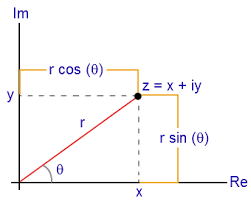
\includegraphics[width=0.5\linewidth]{Argand_plane}
	\caption{The Argand Plane.}
	\label{fig:argand}
\end{figure}
}

\begin{lemma}
	The Triangle Inequality is:
	$$\norm{z_1 + z_2} \leq \norm{z_1} + \norm{z_2}$$
	We can prove this using the argand representation. 
\end{lemma}

Properties of complex numbers:

\begin{itemize}
	\item Commutative
	\item Associative
	\item Distributive
	\item $z_1 -z_2 = z_1 + (-z_2)$.
	\item $z^n = r^n(\cos(n\theta) + i \sin(n\theta)$
	\item Complex Cojugate: $z^* = \bar{z} = x-iy = r(\cos\theta - i \sin\theta)$
	\item $z z^* = \norm{z}^2$
	\item Division 
\end{itemize}

\Def{Roots of Unity}{Given a complex number $z_0$ characterized by $r_0, \theta_0$, can we find a $z$ such that $z^n = z_0$? Well, clearly:
$$r^n = r_0$$
$$\cos(n\theta) + i \sin(n\theta) = \cos(\theta_0) + i \sin(n\theta_0)$$

This, $\norm{z} = r_0^{1/n}$, and $n\theta = \theta_0 + 2k\pi,\ k = 0, \pm 1, \pm 2...)$ There are only $n$ different solutions, meaning there are only $n$ roots. If we let $z_0 = 0$, we can find the roots of unity:

$$\text{roots of unity} = z = \cos(\frac{2k\pi}{n}) + i \sin(\frac{2k\pi}{n})$$
If we let $\omega = \cos(\frac{2\pi}{n}) + i \sin(\frac{2\pi}{n})$, then $\sum_{k=0}^{n-1} \omega^k = 0$

TODO: rebecca, this seems a bit wrong. See \href{https://en.wikipedia.org/wiki/Root_of_unity}{https://en.wikipedia.org/wiki/Root\_of\_unity} for a better explanation.

Essentially, geometrically, this means that the powers of $\omega$ sum to zero, as in Figure \ref{fig:3rdrootsofunity}.

\begin{figure}[H]
	\centering
	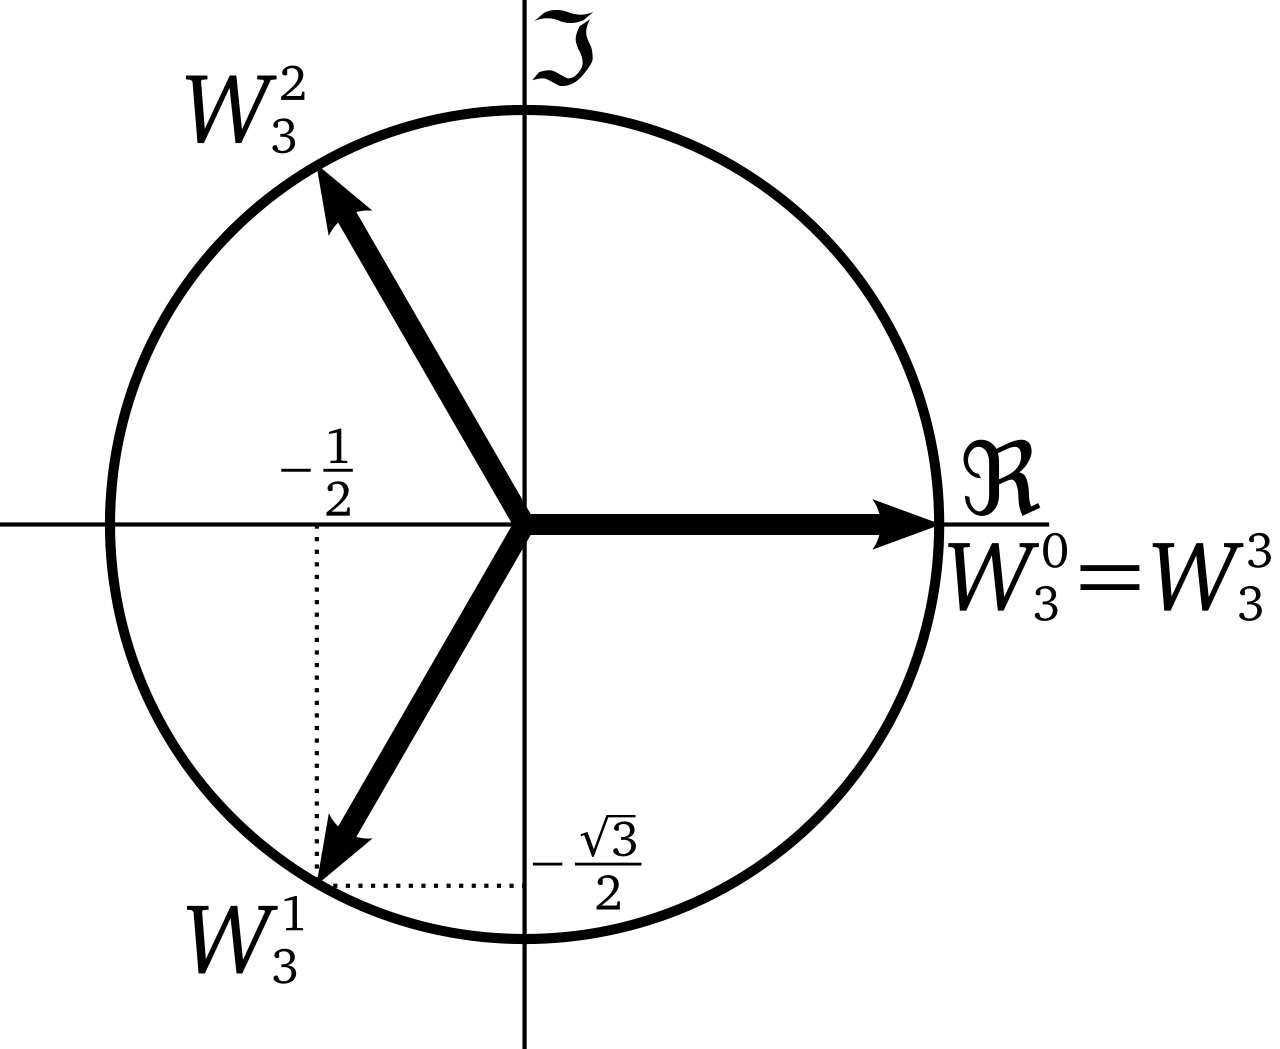
\includegraphics[width=0.5\linewidth]{3rd_roots_of_unity}
	\caption{The third roots of unity sum to one - as do nth roots of unity. \textit{Wikipedia.}}
	\label{fig:3rdrootsofunity}
\end{figure}

}

The complex numbers lack the notion of order, in the way the real numbers have order. In particular, the notion of $\infty$ is very different. For real numbers, we have $\pm \infty$, which serves as an upper and lower bound on $\R$. For complex numbers, we define a \textit{point at infinity}. The point at infinity is the limit of what happens as $r$ goes to infinity for $z=r e^{i\theta}$, While it may seem like this goes to a different point for different $\theta$, the point at infinity is in fact the same.

One way to imagine this is to consider the \textit{stereographic projection} (Figure \ref{fig:stereographic}):
\begin{figure}[H]
	\centering
	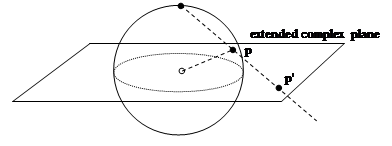
\includegraphics[width=0.5\linewidth]{stereographic_projection}
	\caption{The stereographic projection. We can see that as the point picked to move away from the point at infinity (the north pole), becomes horizontal. The intersection point on the sphere will gradually move closer to the point at the north pole, hence the north pole is the point at infinity. \textit{MathPages}.}
	\label{fig:stereographic}
\end{figure}


\subsection{Real and imaginary pairs of Z}

\begin{align*}
	f(z) = u(x,y)+iv(x,y)
\end{align*}

The continuity of $f(z)$ is continuous at $z = x_0 + iy_0$ $\iff u(x,y)$ and $v(x,y)$ are continuous at $x_0, y_0$ 

\subsection{Differentiation of complex functions}

\Def{Differentiable}{A function $f$ is differentiable at point $z$ if 
\begin{itemize}
	\item $\lim_{h\to0} \frac{f(z+h) - f(z)}{h} = f'(z)$ exists
\end{itemize}

\textbf{Note:} $h \in \C$ and can approach zero along any path. 
}


\begin{ex}
$f(z) = z^2$ is everywhere differentiable. 
\end{ex}

\begin{ex}
	$f(z) = |z|$ is continuous, but not differentiable at $z = 0$. 
	
	If we look at the definition:
	
	$\lim_{h\to0} \frac{f(z+h) - f(z)}{h} = \lim \frac{|h|}{h}$
	
	but $|h|$ approaches 0 so the limit does not exist.
\end{ex}



\begin{theorem}[Differential of a Complex function]
\begin{enumerate}
	\item If $f(z) = z^m$, m is integer, then $f'(z) = mz^{m-1}$
\end{enumerate}
If $f(z)$ and $g(z)$ are differentiable, then:
\begin{enumerate}
	\item$(f+g)' = f'+g'$
	\item$(fg)' = f'g + fg'$
	\item$(f/g)' = \frac{f'g-fg'}{g^2},\ g \neq 0 $
\end{enumerate}


Suppose g is differentiable at z and f is differentiable at g(z). If F(z)=f(g(z)), then:

$$ F'(z) = f'(g(z))g'(z)$$

Suppose that $h \to 0$ along the real axis. Then:

\begin{align*}
\frac{f(z+h) - f(z)}{h} & = \frac{u(x+h, y) + iv(x+h,y) - u(x,y) - iv(x,y)}{h}\\
& = \frac{u(x+h, y) - u(x,y) }{h} + i \frac{v(x+h,y) v(x,y)}{h}
\end{align*}

If f is differentiable at z = x+iy, both limits (as $h \to 0$) must exist and:

$$f'(z) = \frac{\partial u}{\partial x} + i  \frac{\partial v}{\partial x}$$

Next, suppose that h = ik, $k \in \R$.

\begin{align*}
\frac{f(z+h) - f(z)}{h} & = \frac{u(x, y+k) + iv(x,y+k) - u(x,y) - iv(x,y)}{ik}\\
& = \frac{u(x, y+k) - u(x,y) }{ik} + i \frac{v(x,y+k) v(x,y)}{ik}
\end{align*}

Since f is differentiable, both limits as $k \to 0$ must exist. We can conclude that:

$$f'(z) = \frac{\partial v}{\partial y} - i  \frac{\partial u}{\partial y}$$

We conclude that:


$$\boxed{f'(z) = \frac{\partial u}{\partial x} + i  \frac{\partial v}{\partial x} = \frac{\partial v}{\partial y} - i  \frac{\partial u}{\partial y}}$$


We can additionally conclude the \textbf{Cauchy-Riemann Conditions}:

$$\frac{\partial u}{\partial x} = \frac{\partial v}{\partial y},\ \frac{\partial v}{\partial x} = -\frac{\partial u}{\partial y}$$

\end{theorem}

\Def{Cauchy-Riemann Equations}{For a function $f(z) = u(x,y)+iv(x,y)$:
	$$\frac{\partial u}{\partial x} = \frac{\partial v}{\partial y},\ \frac{\partial v}{\partial x} = -\frac{\partial u}{\partial y}$$
	
	These furnish a necessary condition for differentiability at a point.
	
	\begin{remark}
		The Cauchy-Riemann equations are necessary, but \textbf{not} sufficient for differentiability at a point.
\end{remark}}

\begin{ex} Consider the complex conjugate function:
	$$f(z) = z^* = \bar{z} = x-iy$$
	
	We would like to determine if $f$ is differentiable. If it is, it must satisfy Cauchy-Riemann equations.
	
	$$\frac{\partial u}{\partial x} = 1,\ \frac{\partial v}{\partial y} = -1$$
	
	Already, we see that $\frac{\partial u}{\partial x} \neq \frac{\partial v}{\partial y}$. So $f(z)$ is not differentiable for any value of z.
\end{ex}

\begin{remark}
The Cauchy-Riemann equations can also be written as:

$$f'(z) = \frac{\partial f}{\partial x} = -i \frac{\partial f}{\partial y}$$

\end{remark}


\begin{theorem}
	Let $f=u+iv$ be differentiable with complex partials at $z=re^{i\theta}$. Then:
	$$\pdv{u}{r} = \frac{1}{r} \pdv{v}{\theta},\ \pdv{v}{r} = -\frac{1}{r} \pdv{u}{\theta}$$
\end{theorem}


\Def{Analyticity}{A function is \textbf{analytic (holomorphic) }at a point if it is differentiable everywhere in some neighborhood of the point. If the function is analytic for all values of $z \in \C$, then it is \textbf{entire}. 
	
Note: Being differentiable in a neighborhood (analytic) is a stronger requirement than just differentiable. 

\textbf{Remark:} If a function is analytic at a point, it is differentiable for all orders at that point.
}


\begin{ex} Let 
$f(z) = |z|^2 = z \bar{z}$. This function is differentiable only at $z=0$, but it is nowhere analytic. 
\end{ex}

\begin{theorem}Let $f(z) = u(x,y)+iv(x,y)$  be defined in a domain D. Let $u(x,y)$ and $v(x,y)$ have continuous partials that satisfy Cauchy-Riemann equations for all points in D. Then, we can show that $f(z)$ is analytic in D. Thus, Cauchy-Riemann applied to the neighborhood is sufficient to show analyticity.
\end{theorem}

\begin{ex}
$f(z)=e^z = e^z=e^x(\cos y + i \sin y)$


Therefore, $e^z$ is an entire function. 

$$f'(z) = e^z$$
\end{ex}

Note: if $f$ is analytic of non-zero at a point z, then a branch may be chosen for which $\log (f(z))$ is also analytic in the neighborhood of z and $\dv{}{z} log(f(z)) = \frac{f'(z)}{f(z)}$


\subsection{Branch points and Branch Cuts}
Explaining the epsilon method: \url{https://math.stackexchange.com/questions/2150639/branch-point-of-logz}
The easy way to do branch points is to remember that $log(z)$ and $z^p$ where p is non integer both have branch points at $0, \infty$. So simply find when $z = 0, \infty$ for those functions to get the branch points. Then a branch cut must connect all branch points, but does not have to go in any particular way. For $log(z)$, the negative real line is often the branch cut that is picked.


Branch points are points where the function is non-analytic. 

\subsection{Harmonic functions}
Later, we will see that analytic functions have derivatives of all orders. Recall:
$$f'(z) = \frac{\partial f}{\partial x} = -i \frac{\partial f}{\partial y}$$

We can take the derivative:

$$f''(z) = \frac{\partial f}{\partial x} = -i \frac{\partial f}{\partial y}$$
And so:
$$\pdv{^2f}{x^2} + \pdv{^2f}{y^2} = 0$$

Since $f(z) = u(x,y) + i v(x,y)$, 

$$\pdv{^2u}{x^2} + \pdv{^2u}{y^2} = 0 \pdv{^2v}{x^2} + \pdv{^2v}{y^2} = 0$$

\Def{Harmonic Function}{ A continuous, real valued function u(x,y) defined on domain D is called \textbf{harmonic} if it has continuous first and second derivatives, satisfying Laplace's equation:
$$\pdv{^2u}{x^2} + \pdv{^2u}{y^2} = 0$$ 

Note: The real and imaginary parts of an analytic functions are harmonic functions.}

\Def{Harmonic Conjugate}{If $f(z) = u + iv$ is analytic, $v$ is called the harmonic conjugate of $u$, and vice versa.}

\begin{remark}
Laplace's equation furnishes a \textbf{necessary} condition for a function to be real and imaginary parts of an analytic function.
\end{remark}

\begin{ex}
$u(x,y) = x^2+y$

This cannot be the real part of any analytic function, since the Laplace equations are not satisfied. $$\pdv{^2u}{x^2} + \pdv{^2u}{y^2} \neq 0 $$.
\end{ex}

\Section{Sequences}
\Def{Sequence}{ A sequence $\{z_n\}$ of complex numbers is an assignment of a complex number $z_n$ to each positive integer $n$.}

\Def{Convergent sequence}{A sequence $\{z_n\}$ is said to have a limit $z_0$ or converge to $z_0$ which we write as 

$$\lim_{n\to\infty} z_n = z_0$$

if for every $\epsilon > 0, \exists\ M \in  \mathbb{Z}$, such that:

$$|z_n - z_0| < \epsilon,\ \forall n > M$$

This means for sufficiently large values of $n$, $z_n$ is arbitrarily close to $z_0$.

\begin{figure}[H]
	\centering
	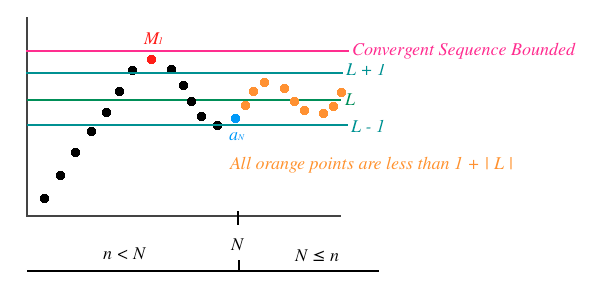
\includegraphics[width=0.7\linewidth]{convseq}
	\caption{A convergent sequence example. }
	\label{fig:convseq}
\end{figure}

Alternative definition: Every neighborhood of $z_0$ contains all but a finite number of $z_n$'s.
}

\begin{ex}
$\{\frac{1}{m}\}$ converges to 0. However, $\{(-1)^{m}\}$ does not converge. 
\end{ex}

\begin{theorem}
Let $z_m = x_m + i y_m$ be a sequence of complex numbers $\{z_m\}$. Then, this converges to $z_0 = x_0 + i y_0$ if and only if the real sequences $\{x_m\}, \{y_m\}$ converge to $x_0, y_0$ respectively.

\textbf{Remark}: The properties of complex sequences can be derived from corresponding properties of real sequences. For example, the uniqueness of the limit (can only converge to one value).
\end{theorem}

\begin{theorem}
A convergent sequence is bounded. 

\textbf{Proof:}

If $\lim_{m\to\infty}z_m = z_0$, then there must be a $z_m \in N(z_0,1)$ , where $N$ means neighborhood, for $m>N$, let $M = \max\{|z_1|, .., |z_N|\}$, then
$$|z_m| < M + |z_0| + 1, \forall m$$

Note that the converse is not true. Counterexample:

$\{1,2,1,2,1,2\}$ is bounded but does not converge. 
\end{theorem}
\Def{Subsequence}{A subsequence of $\{z_m\}$ is a sequence $\{z_{m_k}\}$ whose terms are selected from the terms in an original sequence and arranged in the same order. Subsequences may converge even if sequences do not.}
\begin{ex}
Given a sequence $z_m = (-1)^{m}$, a subsequence could be $z_{m_k} = z_{2k}$, or the even terms, which results in $\{1,1,..1\}$ which converges to 1. The subsequence $z_{m_k} = z_{2k+1}$ converges to -1.
\end{ex}

\begin{theorem}
If a sequence $\{z_m\}$ converges to $z_0$, then every subsequence also converges to $z_0$. 
\end{theorem}

\begin{theorem}
Every bounded sequence of complex numbers contains at least one convergent subsequence. 

\textbf{Proof:} Exercise. 
\end{theorem}

\Def{Cauchy Sequence}{A sequence is Cauchy sequence if in the limit, the difference between the terms becomes arbitrarily small (each value becomes arbitrarily close to each other), which lets us not define the actual limit. 

Formally, a sequence $\{z_m\}$ of complex numbers is a Cauchy sequence if for every $\epsilon>0$, $\exists N \in \mathbb{Z}$ such that $|z_m - z_M| < \epsilon,\ \forall m, M>N$.}

\begin{theorem}
A sequence $\{z_m\}$ converges if and only if $\{z_m\}$ is a Cauchy sequence. 

Note: The two notions of convergence and Cauchy convergence are equivalent. Cauchy convergence is the most general test of convergence. It works even if the limit $z_0$ is not known.
\end{theorem}

\Section{Series}
\Def{Series}{Given a complex sequence $\{a_m\}$, we associate a new sequence defined by $s_m = \sum_{k=1}^{n}a_k$. Then, we say that $\sum_{k=1}^{\infty}a_k$ is a series. The series is said to converge or diverge according to whether the sequence $\{s_m\}$ converges or diverges. We call $\{s_m\}$ the \textbf{partial sum} of the series, and $a_k$ the kth term.

\textbf{Note:} Every theorem about sequences can be rephrased to be a theorem about series, since series are sequences, and vice versa
}
\begin{theorem}
Let $\{a_m\}$ be a sequence of complex numbers, with $a_m = \alpha_m+ i \beta_m$ where $\{\alpha_m\}, \{\beta_m\}$ are sequences of real numbers. Then, by the earlier result, the complex series $\sum_{k=1}^{\infty}a_k$ converges if and only if $\sum_{k=1}^{\infty}\alpha_k$ and $\sum_{k=1}^{\infty}\beta_k$ converge.
\end{theorem}


\Def{Cauchy Criterion.}{Let $s_m = \sum_{k=1}^{m}a_k$. The series $\sum_{k=1}^{\infty}a_k$ converges if and only if for every $\epsilon>0$, there exists $N \in \mathbb{Z}$ for $m, M>N$:

$$|s_M - s_m| = \left|\sum_{k=m+1}^{M}a_k\right| < \epsilon$$

Alternatively, letting $M = m+p$:

$$|s_{m+p} - s_m| = \left|\sum_{k=m+1}^{m+p}a_k\right| < \epsilon, \forall p = 1,2,3,..$$

This is the most general test for convergence of a series. 

Note: Familiar properties of a series are immediate consequences of the Cauchy criterion.

Note: $a_k \to 0$ to converge. (set $p=1$).
 }

\Def{Absolutely Convergence}{A series $\sum_{m=1}^{\infty}a_m$ is said to be absolutely convergent if $\sum_{m=1}^{\infty}|a_m|$ converges. 

\textbf{Note:} Applying the triangle inequality:

$$\left|\sum_{k=m+1}^{m+p}a_k\right| \leq \sum_{k=m+1}^{m+p}\left|a_k\right|$$

Applying this with the Cauchy criterion, we can deduce that absolute convergence of a series ensures its convergence. 

\textbf{Note:} If $|a_m| \leq |b_m|$, for every $m$, the convergence of $\sum_{m=1}^{\infty} |b_m|$ implies convergence of $\sum_{m=1}^{\infty} |a_m|$ .
}

\begin{theorem}
Suppose $a_m>0\ \forall m$ and that $\sum_{m=1}^{\infty} a_m$ diverges. If $s_m = \sum_{k=1}^m a_k$, then:
\begin{enumerate}
	\item $\sum_{m=1}^{\infty} \frac{a_m}{s_m}$ also diverges.
	\item $\sum_{m=1}^{\infty} \frac{a_m}{s_m^2}$ also converges. This is shown by Cauchy. 
\end{enumerate}
\end{theorem}

\begin{corollary}
The series 	$\sum_{m=1}^{\infty} \frac{1}{m}$ also diverges. But $\sum_{m=1}^{\infty} \frac{1}{m^2}$ converges.
\end{corollary}

\begin{theorem}[Geometric series]
Consider $s_m = \sum_{k=1}^m r^{k-1} = \frac{1-r^m}{1-r}$. This is a geometric series.  

\textbf{Proof:}

\begin{align*}
(1-r)\sum_{k=1}^m r^{k-1} &= \sum_{k=1}^m r^{k-1} - r^k \\ 	
& = 1-r^m
\end{align*}

Hence a series $\sum_{m=1}^\infty a_m$ converges absolutely if ther eexists a constant $r \in [0,1)$ and a real number M such that $|a_m| < M r^m,\ m>M$
\end{theorem}

\subsection{Limits of series and sequences}
\Def{Limit Superior }{Let $\{a_m\}$ be the real bounded sequence and let A be the set of subsequence limits of $\{a_m\}$. We define the limit $\sup$ of $\{a_m\}$ as the least upper bound of A:

$$\lim\sup_{m \to \infty }a_m = L.U.B.\{A\}$$

\textbf{Note:} If $\{a_m\}$ is unbounded above, then:

$$\lim\sup_{m \to \infty }a_m = + \infty $$


Note: If all but a finite number of $a_m$ are less than any pre-assigned real number, we say that :

$$\lim\sup_{m \to \infty } a_m = - \infty $$
}



\Def{Limit Inferior}{Let $\{a_m\}$ be the real bounded sequence and let A be the set of subsequence limits of $\{a_m\}$. We define the limit $\inf$ of $\{a_m\}$ as the greatest lower bound of A:
	
	$$\lim\inf_{m \to \infty }a_m = G.LB.\{A\}$$
}

Note: in the extended reals $(\R \cup \pm \infty)$, the limit superior and limit inferior of a real sequence always exists. This allows us to state and prove results without worrying about the existence of limits.

\begin{theorem}
Let $\{a_m\}$ and $\{b_m\}$ be real valued sequences. Then, 
\begin{enumerate}
	\item $\lim \sup_{m \to \infty }(a_n + b+m) \leq \lim\sup a_m + \lim\sup b_m$
	\item $\lim \inf_{m \to \infty }(a_n + b+m) \leq \lim\inf a_m + \lim\inf b_m$
\end{enumerate}
\end{theorem}

\begin{remark}
\textbf{On the difference between limsup and sup}
\url{https://math.stackexchange.com/questions/1734087/difference-between-limsup-and-sup}

\end{remark}

\begin{theorem}[Root Test]
Let $\{a_m\}$ be a complex sequence and suppose that:
$$\lim\sup_{m \to \infty } |a_m|^{1/m} = L$$

Then the series $\sum_{m=1}^\infty a_m$ converges absolutely if $L<1$ and diverges if $L>1$. 

\textbf{Proof:}

Case 1: \\ 
If $L<1$, choose $r$ such that $L<r<1$. For all but a finite number of m, we have that:

\begin{align*}
|a_m|^{1/m} & < r \\ 
|a_m|&  < r^m  
\end{align*}

This is true since by the definition of $L$, this must be true. 

The convergence of $\sum_{m=1}^\infty a_m$ now follows from convergence of $\sum_{m=1}^\infty r^m$, $r<1$.

Case 2:\\
If $L>1$, then $|a_m|^{1/m} >1$ for infinitely many values of $m$. But then $|a_m|>1$ infinitely often. Then $a_m \not \to 0$ and the series diverges. 

Case 3: \\ 
If $L=1$, the root test does not give any information.

\textbf{Ex:} $\sum \frac{1}{m}$ diverges, but $\sum \frac{1}{m^2}$ converges.

 However, $\lim\sup_{m \to \infty }|\frac{1}{m}|^{1/m} = 1$. Similarly, $\lim\sup_{m \to \infty }|\frac{1}{m^2}| = 1$

\end{theorem}

\subsection{Convergence}
\Def{Pointwise Convergence}{A sequence of functions $\{f_m(z)\}$ converges pointwise to a function $f$ on a set $E$ $(f_m \to f)$, if to each $z_0 \in E$, and $\epsilon>0$, there corresponds  and integer $N = N(\epsilon, z_0)$ for which $|f_m(z_0) - f(z_0)|<\epsilon$ whenever $m>N$.

Pointwise convergence implies $\lim_{m\to\infty} f_m(z_0) = f(z_0)$


Note: the integer $N$ may, in general, vary with $z_0 \in E$. If one integer can be found that works for all $z_0 \in E$, then we have a special (stronger) type of convergence: \textbf{uniform convergence.}
}

\Def{Uniform Convergence}{A sequence of functions $\{f_m\}$ converges uniformly to $f$ on set $E$ $(f_m \Rightarrow f)$, If for each $\epsilon>0$ there corresponds an integer $N = N(\epsilon)$ such that for all $z \in E$, $|f_m(z_0) - f(z_0)| < \epsilon$ whenever $m>N$.}

\begin{ex}
Consider $f_m(z) = \frac{1}{mz}$ . This converges pointwise but not uniformly to $f(z)=0$ in the set $0<|z|<1$. This is because uniform convergence would require existence of $N$ such that $\left|\frac{1}{mz}\right| < \epsilon < 1$ valid for all $z$ in the set. You can see this is not true in the case $z = \frac{1}{n}$. $f(\frac{1}{n})$ would be greater than $1$, so yeah. 
\end{ex}

The importance of uniform convergence is that it allows for the interchange of many limiting operations.  which, in turn, compels the limit to retain many properties of sequences.

\begin{theorem}
Suppose $\{f_m\}$ converges uniformly to $f$ on $E$. If each $f_m$ is continuous at point $z_0 \in E$, the limit of the function $f$ is also continuous at $z_0$:

$$\lim_{z \to z_0} \lim_{m \to \infty }f_m(z) = \lim_{m \to \infty }\lim_{z \to z_0}f_m(z)$$


The provides a necessary condition for uniform convergence.
\end{theorem}

\begin{ex}
$f_m = \frac{1}{1_mz}$. This converges pointwise to 

\begin{align*}
f = \begin{cases}
0 & if\ z\neq 0 \\ 1 & if\ z = 0 \\ 
\end{cases}
\end{align*}

Since $f$ is not continuous, the convergence cannot be uniform in any region containing the point $z=0$. 
\end{ex}

Note, this generalizes cauchy convergence. 



\subsection{Series of Complex Functions}
Given a sequence of functions $\{f_m\}$ defined on the set $E$, we associate a new sequence $\{s_m(z)\}$ defined by 
$$s_m(z) = \sum_{k=1}^m f_m(z)$$

For values for which  $\lim_{m \to \infty }s_m(z)$ exists, we say the series converges. 

\begin{align*}
f(z) &= \lim_{m \to \infty } \sum_{k=1}^m f_k(z) \\ 
& = \sum_{k=1}^\infty f_k(z)
\end{align*}

Note, this is different than before. Now $f(z)$ is the limit of the sum, not just the limit.

If $\{s_m(z)\}$ converges uniformly on $E$, then the series $\sum_{k=1}^\infty f_k(z)$ is said to be \textbf{uniform} on $E$. Similarly, if $\sum_{k=1}^\infty f_k(z)$ is uniformly convergent on $E$, then
$\sum\left|f_m(z)\right|$ converges. 

\begin{theorem}
The series $\sum_{m=1}^\infty f_m(z)$ converges uniformly on a set $E$ if and only if to each $\epsilon$, there corresponds an integer $N = N(\epsilon)$, such that for all $z \in E$, 
\begin{align*}
\left|\sum_{k=m+1}^{m+p}f_k(z) \right| < \epsilon,\ m>N,\ p = 1,2,3..
\end{align*}


By the triangle inequality, this also implies absolute convergence. 
\end{theorem}

\begin{theorem}[Weirstrass M-test]
Let $M_m$ be a sequence of real numbers. Suppose that $|f_m(z)| < M_m, \forall z \in E, m\in \mathbb{Z}^+$.  If $\sum_{m=1}^\infty M_m$ converges, then $\sum_{m=1}^\infty f_m(z)$ converges uniformly and absolutely on $E$. 
\end{theorem}
\begin{ex}
The series $\sum_{m=1}^\infty z^m $ converges absolutely for $|z|<1$. It converges uniformly for $|z|\leq r < 1$. 
\end{ex}

Note: $\sum_{m=1}^\infty |z^m| = \sum_{m=1}^\infty |z|^m = \frac{|z|}{1-|z|},\ |z|<1$. This proves absolute convergence for $|z|<1$. 


Let $M_m = r^m$. Then $|z^m| \leq r^m$ for $|z| \leq r < 1$. But $\sum_{m=1}^\infty r^m$ converges for $r<1$. So: $\sum_{m=1}^\infty z_m$ converges uniformly for $|z| \leq r < 1$. This follows from the Weirstrass M-test. 

\Section{Power Series}
\Def{Power Series}{Let $f_m(z) = a_m(z-b)^m$ where $a_m, b$ are complex. $\sum_{m=1}^\infty f_m(z) = \sum_{m=0}^\infty a_m(z-b)^m$ is a called a power series in $z-b$. WLOG, set $b=0$. }

\begin{theorem}
Suppose a power series $\sum_{m=0}^\infty a_m z^m$ converges at point $z=z_0$. Then $\sum_{m=0}^\infty |a_m| |z|^m$ converges for $|z|<|z_0|$. 

Basically, if it converges at $z_0$, then it converges in a disc centered at $b$ with radius $z_0-b$. 

\textbf{Proof:} Since $\sum_{m=0}^\infty a_m z_0^m$ converges, we have that $\lim_{m \to \infty }a_m z_0^m = 0$. Hence there is a constant $M$ such that $\left|a_mz_0^m\right|<M,\ \forall m$. Also:

$$|a_m| |z|^m =\left| a_m z_0^m \left(\frac{z}{z_0}\right)^m \right| < M \left|\frac{z}{z_0}\right|^m$$
For $|z|<|z_0|$, the geometric series $\sum_{m=0}^\infty \left|\frac{z}{z_0}\right|^m$ converges. Thus:

$$\sum_{m=0}^\infty |a_m| |z|^m \leq \sum_{m=0}^\infty \left|\frac{z}{z_0}\right|^m = \frac{M}{1-\left|\frac{z}{z_0}\right|},\ |z|<|z_0|$$
\end{theorem}

\begin{corollary}
If $\sum_{m=0}^\infty a_m z^m$ diverges at $z = z_0$, then $\sum_{m=0}^\infty a_m z^m$ diverges for $|z| > |z_0|$. 
\end{corollary}

\begin{corollary}
Of $\sum_{m=0}^\infty a_m z^m$ converges for all real values of z, then the series also converges for all complex values.	\end{corollary}
\begin{theorem}
For every power series $\sum_{m=0}^\infty a_m z^m$, there correspondes a number $R \in [0, \infty]$ for which it satisfies:
\begin{enumerate}
	\item It converges absolutely in $|z| < R$
	\item It converges uniformly in $|z|\leq R_0 < R$ 
	\item It diverges for $|z|>R$.
\end{enumerate}

\textbf{Proof:} Let $s = \{r\ s.t.\ \sum_{m=0}^\infty a_m z^m\text{ converges for } |z|<r\}$. Then $R = \begin{cases}
L.U.B. s \text{ if } s \text{is bounded} \\ 
\infty \ otherwise
\end{cases}$

Note: $R$ is the radius of convergence of a power series. It converges inside, diverges outside the circle $|z| = R$. On the other hand, it may converge at all some, or none of the points on the circle $|z|=R$. 

\end{theorem}

\begin{theorem}
The power series $\sum_{m=0}^\infty a_m z^m$ has a radius of convergence $R = \frac{1}{A}$, where $A =\lim\sup_{m \to \infty } |a_m|^{1/m}$. If $A = \infty$, $R = 0$. Likewise, if $A=0$, $R = \infty$. 

\textbf{Proof:}
For any point $z_0$, $\lim\sup_{n \to \infty } |a_nz_0^n|^{1/n} = \left(\lim\sup_{n \to \infty }|a_n|^{1/n}\right)$. According to the root test, the series $\sum_{m=0}^\infty a_m z^m$ converges absolutely when $|z_0|A < 1$ 

\textbf{Note:} $f(z) = \sum_{m=0}^\infty a_m z^m$ is continuous at $z = z_0$ with $|z_0|<R$. what about differentiation?
\end{theorem}


\begin{theorem}
If a function $f(z)$ is the pointwise limit of a power series $\sum_{m=0}^\infty a_m z^m$ in $|z|<R$,
\end{theorem}
See other notes of 9/23-9/25 for a description of what happened here.

\Section{Contours}

Note: If f is analytic in domain including $C$, we can find $F$ such that $F'=f$

\begin{theorem}[Cauchy's Theorem]
If $f(z)$ is analytic in a Domain D and C is a closed contour lying on D, then $$\int_{C} f(z) dz = 0$$

\textbf{Note:} the argument use to generalize the weaker version of Cauchy for multiply connected regions can be repeated for the stronger version

\textbf{Note:} this takes the work of parameterizing ugly contours, as will be seen in the next example.
\end{theorem}

\begin{ex}
Evaluate $\int_C \frac{1}{z-z_0}dz$ for some arbitrary ugly contour
Define a nice contour $C_1 : |z-z_0| = \epsilon$ which is a circle completely inside $C$, such that it does not divide the interior region.

Now, $f(z) = \frac{1}{z-z_0}$ is analytic in a multiply connected region between $C$ and $C_1$. Hence
$$\int_{C+C_1}f(z)dz = 0$$

Therefore, $\int_C \frac{1}{z-z_0}dz = -\int_{C_1} \frac{1}{z-z_0}dz$. 

Since $C_1 : z(t) = z_0 + \epsilon e^{it},\ t \in [0, 2\pi]$. Thus, 

$$\int_C \frac{1}{z-z_0}dz = \int_{0}^{2\pi}\frac{z'(t)}{z(t)-z_0} dt = \int_{0}^{2\pi} \frac{i\epsilon e^{it}}{\epsilon e^{it}} dt = 2\pi i$$
\end{ex}

\Def{Laplace Transform}{$$F(s) = \int_{0}^{\infty} e^{-st} f(t) dt$$

The inversion of the Laplace transform involves an integral on the complex plane of a vertical contour to the right of all singularities. 

$$f(t) = \frac{1}{2\pi}\int_{\gamma - i \infty}^{\gamma + i \infty} F(s) e^{st}ds $$

There is a trick where you can close the contour to the right if there are no singularities to the right of the contour. Then, this causes $f(t)$ to have a zero contribution from the point at infinity. This only happens if $t<0$. This is usually true as $f(t)$ is usually zero before $t=0$.}


\begin{theorem}[Cauchy Integral Formula]
	
Let $f(z)$ be analytic in a simply connected domain containing the simple closed contour C. If $z_0 \in C$, then 

$$f(z_0) = \frac{1}{2\pi i}\int_{C} \frac{f(z)}{z-z_0}dz$$

\begin{figure}[H]
	\centering
	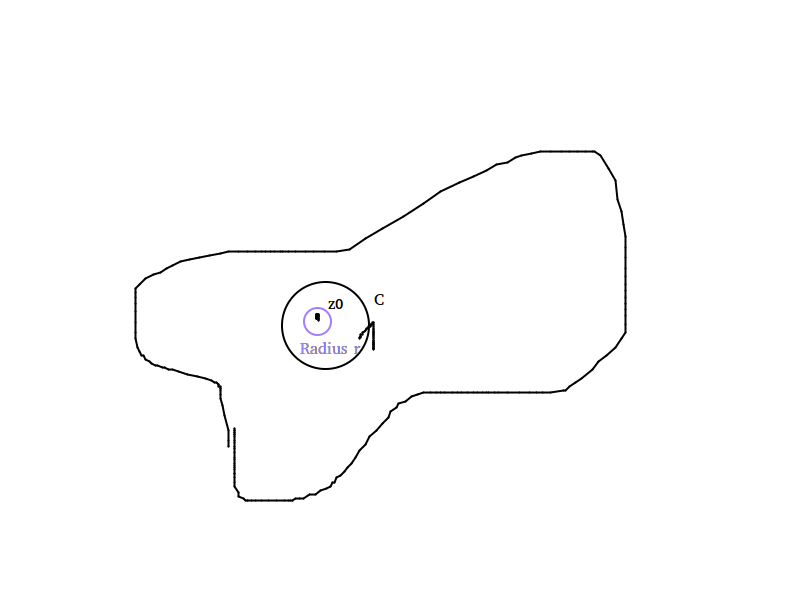
\includegraphics[width=0.7\linewidth]{intform}
	\caption{Contour for Cauchy integral Form on some domain.}
	\label{fig:intform}
\end{figure}

Note: $f(z)=1$ is the previous example.

Roughly speaking, if $z_0$ in the integral, then $\frac{f(z)}{z-z_0}dz = 2\pi i f(z_0)$. If it is outside $C$, the value of the integral is zero. 

\textbf{Proof:}

Given $\epsilon>0$, construct a circle $C_1: |z-z_0|=r$. And small enough $r$ such that $|f(z) - f(z_0)|<\epsilon$ for all $z$ on $C_1$. By Cauchy's theorem:

\begin{align*}
\int_C \frac{f(z)}{z-z_0}dz &= \int_{C_1} \frac{f(z)}{z-z_0}dz\\ 
& = \int_{C_1} \frac{f(z_0)}{z-z_0}dz +  \int_{C_1} \frac{f(z) - f(z_0)}{z-z_0}dz\\
 & = 2 \pi i f(z_0) +  \int_{C_1} \frac{f(z) - f(z_0)}{z-z_0}dz
\end{align*}

However:

\begin{align*}
\left|\int_{C_1} \frac{f(z) - f(z_0)}{z-z_0}dz \right| &\leq \int_{C_1} \frac{|f(z) - f(z_0)|}{|z-z_0|}dz \\
&< \int_{0}^{2\pi} \frac{\epsilon}{r} |dz| = \epsilon 2 \pi 
\end{align*}

This goes to zero as $\epsilon \to 0$. Thus, $\int_C \frac{f(z)}{z-z_0}dz = 2 \pi i f(z_0)$

\textbf{Note:} The theorem expresses the value of $f(z)$ at any point in $C$ in terms of values of $f$ on $C$ (no real valued analog to this result).
\end{theorem}

\begin{theorem}[Cauchy Integral Formula for Derivative]
Let $f(z)$ be analytic on a simply connected domain containing a closed simple contour $C$. Then, $f(z)$ has derivatives of all orders at each point $z_0 \in C$. Moreover, the $nth$ derivative at that point is:
$$f^{(n)}(z_0) = \frac{n!}{2\pi i } \int_C \frac{f(z)}{(z-z_0)^{n+1}}dz$$

\textbf{Proof:}
Use the previous result with the definition of the derivative. Assume that $h$ is small enough such that $z_0+h$ is inside $C$. Then:

\begin{align*}
\frac{f(z_0+h) - f(z_0)}{h}& = \frac{1}{2\pi i h } \left(\int_C \frac{f(z+h)}{z-z_0-h} dz - \int_C \frac{f(z)}{z-z_0}dz \right)\\
&= \frac{1}{2\pi i } \int_C \frac{f(z)}{(z-z_0)(z-z_0-h)} dz
\end{align*}

As $h \to 0$, we see $f'(z_0) = \frac{1}{2\pi i h } \int_C \frac{f(z)}{(z-z_0)^2} dz$. However, it is hard to take the limit of an integral so this is hard, so we have to argue this.
\end{theorem}

\textbf{Note:} We know by hypothesis that $f(z)$ was differentiable at all $z_0$ inside $C$. The theorem demonstrates the existence of all derivatives of $f(z)$. 

\textbf{Note:} If $f$ is analytic at $z_0$, it is differentiable to all orders there. 

\textbf{Note:} The Cauchy-integral formula is also valid for multiply connected domains.

\begin{ex}
\begin{figure}[H]
	\centering
	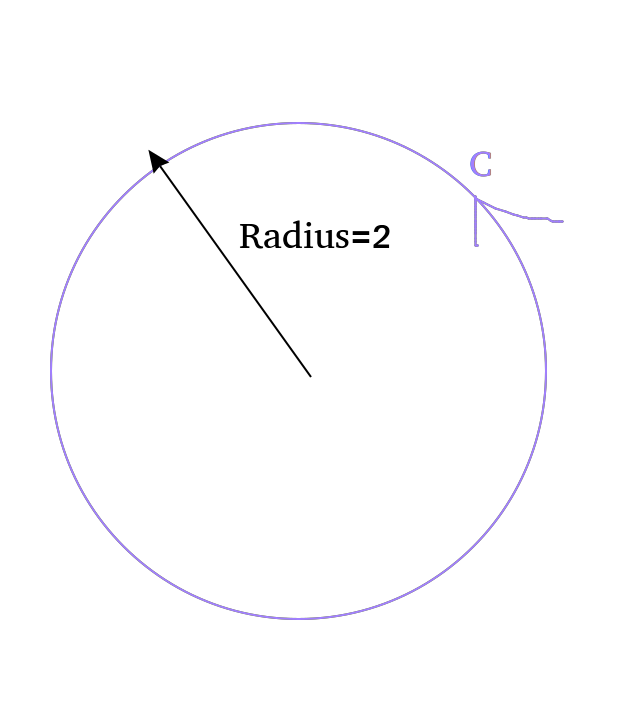
\includegraphics[width=0.4\linewidth]{example12}
	\caption{}
	\label{fig:example12}
\end{figure}


$$\int_{|z|=2}\frac{z-3\cos z}{(z-\pi/2)^2}dz$$

Let $f(z) = z-3\cos z$. Then $f'(z) = 1+3 \sin z$. By the Cauchy integral Formula, 

$$\int_{C} \frac{f(z)}{(z-z_0)^2} dz = 2\pi i f'(\pi/2) = 8\pi i $$
\begin{quote}
	"Almost like magic, isn't it?"
\end{quote}
\end{ex}


\Def{Principal Value Integrals}{
If $z_0$ is outside contour $C$, then $\frac{1}{2\pi i}\int_{C} \frac{f(z)}{z-z_0}dz = 0$. If $z_0$ is on $C$, the integral does not exist. Instead, the integrand blows up "too strongly." However, we can re-interpret the integral so as to avoid the singularity, keeping in mind of course that such a reinterpretation is a matter of definition. Given $C$ and $z_0$ through $C$, and not having a corner there , we consider the modified contour $C'$ excluding $z_0$, putting $z_0$ on the inside. By semi-circle of radius $\epsilon>0$. Then:

$$\frac{1}{2\pi i}\int_{C'} \frac{f(z)}{z-z_0}dz = 0$$

As $\epsilon \to 0$, the part over the semicircle becomes 

$$\frac{1}{2\pi i}\int_{\pi}^0 \frac{f(z_0 + \epsilon e^{i\theta})}{\epsilon e^{i\theta}} i \epsilon e^{i\theta} d\theta = -\frac{f(z_0)}{2}$$

Using the previous theorems:

$$\frac{1}{2\pi i}\int_{C'} \frac{f(z)}{z-z_0}dz = PV \frac{1}{2\pi i}\int_{C} \frac{f(z)}{z-z_0}dz -\frac{f(z_0)}{2} =  0$$

And so:

$$PV \frac{1}{2\pi i}\int_{C} \frac{f(z)}{z-z_0}dz = \frac{f(z_0)}{2}$$

\textbf{Note:} This relies on putting the contour on the inside, but we could put it on the outside. Key feature, it doesn't matter! Wow. Now if $z_0$ is a corner point enclosing an \textbf{interior angle} of $\alpha$ radians, then the principal value is:

$$PV \frac{1}{2\pi i}\int_{C} \frac{f(z)}{z-z_0}dz = \frac{f(z_0)}{2}$$

\begin{figure}[H]
	\centering
	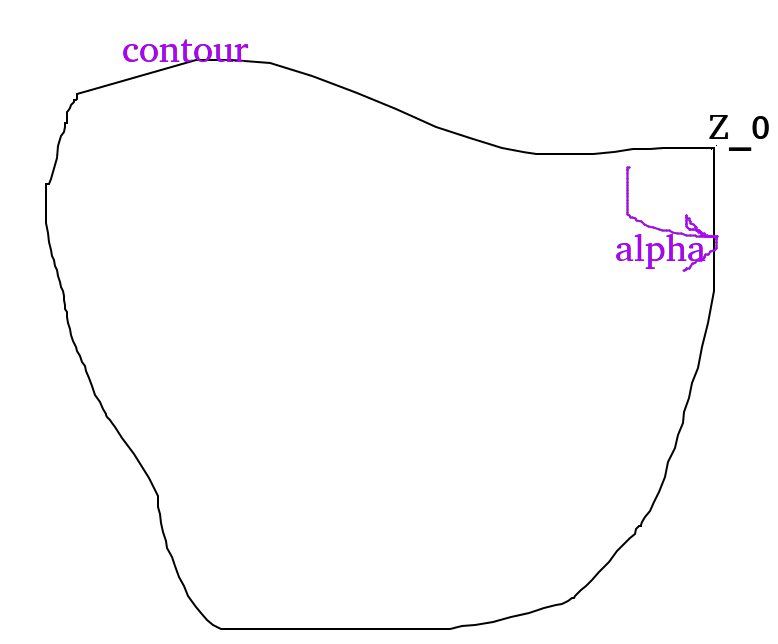
\includegraphics[width=0.5\linewidth]{angle_contour}
	\caption{}
	\label{fig:anglecontour}
\end{figure}

}

% 10/2 Notes
\begin{theorem}[Taylor's Theorem]
Let $f(z)$ be analytic in domain $D$ whose boundary is $C$. If $z_0$ is a point in $D$, then $f(z) = f(z_0) + f'(z_0)(z-z_0) + \frac{1}{2!} f''(z_0) (z-z_0)^2+...$

The series converges for $|z-z_0|<\delta$ where $\delta$ is the distance from $z_0$ to $C$. 

\textbf{Proof:}
\begin{figure}[H]
	\centering
	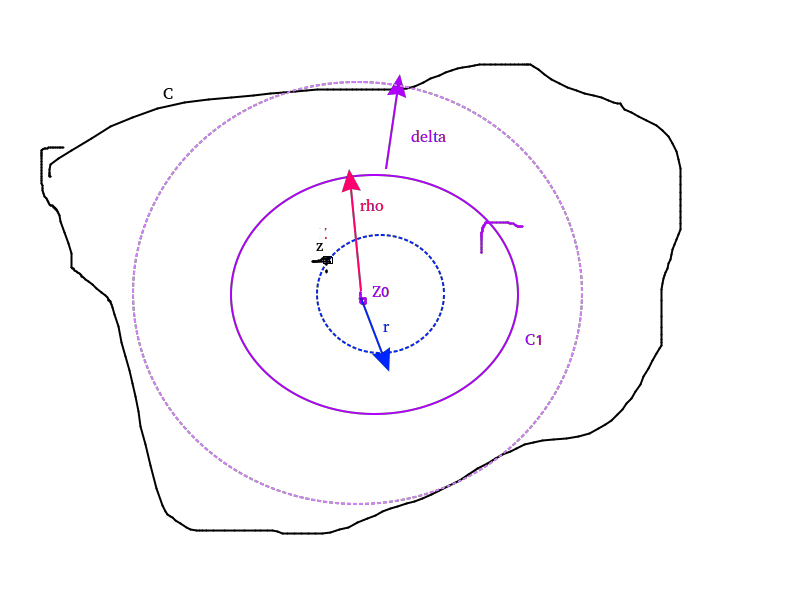
\includegraphics[width=0.5\linewidth]{disc}
	\caption{$\delta$ is the largest circle that fits inside the contour $C$}
	\label{fig:disk}
\end{figure}

Construct circle $C_1:|\zeta - z_0| = \rho$ with $\rho < \delta$. Let $z$ be any point inside $C_1$, then by C.T.M, 

$$\rho(z) = \frac{1}{2 \pi} \int_{C_1} \frac{\rho(\zeta)}{\zeta - z} d\zeta$$.

We set $|z-z_0| = r$, then $ r = |z-z_0|  < |\zeta - z_0| = \rho$. Additionally, 

\begin{align*}
\frac{1}{\zeta - z} &= \frac{1}{\zeta - z_0 - (z - z_0)}\\
&= \frac{1}{\zeta - z_0} \frac{1}{1-\frac{z-z_0}{\zeta - z_0}}\\
&= \frac{1}{\zeta - z_0} \left[1 + \frac{z-z_0}{\zeta - z_0} + \left(\frac{z-z_0}{\zeta - z_0}\right)^2 + .. + \left(\frac{z-z_0}{\zeta - z_0}\right)^{n-1} + \sum_{k=m}^\infty \left(\frac{z-z_0}{\zeta - z_0}\right)^k\right] \\ 
&= \frac{1}{\zeta - z_0} \left[1 + \frac{z-z_0}{\zeta - z_0} + .. + \left(\frac{z-z_0}{\zeta - z_0}\right)^{n-1} + \frac{\left(\frac{z-z_0}{\zeta - z_0}\right)^n}{1-\frac{z-z_0}{\zeta - z_0}}\right]
\end{align*}

Then 

\begin{align*}
f(z) = \frac{1}{2 \pi i } \int \frac{f(\zeta)}{\zeta - z_0} d\zeta + ... + \frac{(z-z_0)^{n-1}}{2 \pi i}\int \frac{f(\zeta)}{\zeta - z_0} d\zeta + R_n
\end{align*}

Where 
$$R_n = \frac{1}{2 \pi i } \int_{C_1} \left(\frac{z-z_0}{\zeta - z_0}\right)^n \frac{f(\zeta)}{\zeta - z}d\zeta$$

By Cauchy Integral Formula, we get that 

\begin{align*}
f(z) = f(z_0) + f'(z_0)(z-z_0) + ... + \frac{f^{(n-1)}(z_0)}{n-1}(z-z_0)^{n-1} + R_n
\end{align*}

However, we still need to show that $R_n \to 0$ as $n \to \infty$. 

%For ??? assume $|f(z)| \leq M $ on $C_1$. Then,
If we instead assume $|f(z)| \leq M $ on $C_1$. Then,
We note that from triangle inequality $$\frac{1}{|\zeta-z|} = \frac{1}{|\zeta - z - z_0 + z_0|} \leq \frac{1}{|\zeta - z_0| - |z-z_0|} = \frac{1}{\rho - r}$$

Then we can conclude that

\begin{align*}
|R_n| &\leq \frac{1}{2 \pi i } \int_{C_1} \left|\frac{z-z_0}{\zeta - z_0}\right|^n \frac{|f(\zeta)|}{|\zeta - z|}|d\zeta \\ 
&\leq \frac{M}{2 \pi i } \left(\frac{r}{\rho}\right)^n \int_{C_1} \frac{1}{|\zeta-z|}|d\zeta| \\
&\leq \frac{M}{2 \pi i } \left(\frac{r}{\rho}\right)^n \frac{1}{\rho - r} 2 \pi \rho 
\end{align*}

Since $r/\rho < 1$ as $n \to \infty$, $|R_n| \to 0$

\textbf{Note:} by the M-test, the Taylor series converges uniformly on  compact subsets of disk $|z-z_0|<\delta$. 


What is this saying? We can chose any circle originating from $z_0$ with radius $R$, as long as it is less than $\delta$ which is the maximum radius to stay within the contour $C$, we will converge uniformly. (is this really true?)
\end{theorem}

We have seen before that a power series represents an analytic function inside its radius of convergence. The result in Taylor's theorem says essentially the converse. Thus, a function $f(z)$ is analytic at a point $z_0$ if and only if $f(z) = \sum_{n=0}^{\infty}a_n(z-z_0)^n$ in some disk $|z-z_0| \leq R$. $a_n$ has a dual representation in both derivative and integral form:

$$a_n  = \frac{f^(n)(z_0)}{n!} = \frac{1}{2 \pi i } \int_{|z-z_0|=\delta} \frac{f(z)}{z - z_0} dz$$


\textbf{Note:} Taylor's theorem now fully justifies Maclaurin expansions such as 

\begin{align*}
e^z &= \sum_{n=0}^\infty \frac{z^n}{n!}\\
\sin z &= \sum_{n=1}^\infty \frac{(-1)^n z^{2n-1}}{(2n-1)!}
\end{align*}


\begin{ex}
Consider $\sum_{n=1}^\infty z^n = \frac{1}{1-z}$. It converges within the disk of radius 1 about the origin.  Can we define the function outside of this disk? This is called \textit{analytic continuation}. We might expand this function around a different point! We see that on the circle $r=1$, the function blows up. How might we do this when we do not know the non-power series form? Contour integrals. More on that later.
\end{ex}

\begin{theorem}
Let $\{f_n(z)\}$ be a sequence of functions continuous on contour $C$. Suppose that the series $\{f_n(z)\}$ converges uniformly to some function $f(z)$ on the contour. Then, we can show that

\begin{align*}
\lim_{n\to\infty} \int_{C} f_n(z) dz &= \int_{C} \lim_{n\to\infty} f_n(z) dz \\ 
&= \int_{C}f(z) dz
\end{align*}

Essentially, this means we can interchange limits, but only for uniformly converging functions.

We can also do this for series: 
\begin{align*}
\sum \int_{C} f_n(z) dz &= \int_{C} \sum f_n(z) dz \\ 
&= \int_{C}f(z) dz
\end{align*}
\end{theorem}

We might expect a function $f(z)$ to be analytic at a point $z_0$ if $\int_{C}f(z)dz = 0$ along every simple closed contour in which $z_0$ is an interior point. However, this is \textbf{NOT TRUE!} 

\textbf{Counterexample:} $f(z) = \frac{1}{z^2}$. 

However, if we add the hypothesis that $f$ is continuous, this is true:

\begin{theorem}[Morera]
Let $f(z)$ be continuous on domain $D$. If $\int_{C}f(z)dz = 0$ along every simple closed contour $C$ contained in $D$, then $f(z)$ must be analytic in $D$. 

\textbf{Proof:}

Fix $z_0$ in $D$, and $F(z) = \int_{z_0}^{z} f(\zeta) d\zeta$. We can consider the derivative of $F$. We can use the continuity of $f$, so it follows that $F$ is analytic.

\end{theorem}

\begin{corollary}
Let $f(z)$ be a function on a simply connected domain $D$. if $z_0$ is a point in $D$, then its integral, $F(z) = \int_{z_0}^z f(\zeta)d\zeta $ is also analytic in $D$. 
\end{corollary}
\begin{theorem}
Let $\{f_n(z)\}$ be a sequence of analytic functions converging uniformly to a function $f(z)$ on all compact (closed and bounded) subsets of a domain $D$. Then, $f(z)$ is analytic in $D$. 
\end{theorem}

\begin{corollary}
Given the same hypothesis as above, $\sum_{k=0}^\infty f_k(z)$ where $f_k(z)$ converges uniformly to $f(z)$ is analytic in $D$.
\end{corollary}

\begin{corollary}
$f'(z) = \sum_{n=0}^\infty f'_n(z)$
\end{corollary}

In the complex case, the term by term differentiation of a sequence of analytic functions uniformly converging on  compact subsets of the domain may be used to get the derivative of the sum. This is not true in the real case.

\begin{ex}
We cannot do term by term differentiation of this real function:
$f(x) = \sum_{n=1}^\infty \frac{\sin(nx)}{n^2}$. Its derivative cannot be computed term by term.
\end{ex}

If $f$ is entire, it has a power series representation of 
\begin{align*}
f(z) = \sum_{n=0}^\infty a_n z^n \\ 
 = \frac{f^(n)(0) z^n}{n!}
\end{align*}
which is valid for all $z$. Then, 

\begin{enumerate}
	\item $f'(z) = \sum_{n=0}^\infty n a_n z^n $
	\item $F(z) = \int_{0}^zf(\zeta)d\zeta = \int_0^z \sum_{n=0}^\infty  a_n \zeta^n d\zeta =\sum_{n=0}^\infty  a_n \int_0^z  \zeta^n d\zeta = \sum_{n=0}^\infty  \frac{1}{n+1} a_n\zeta^{n+1}  $
\end{enumerate}

\begin{ex}
Find the Maclaurin expansion of $f(z) = \log(z+1)$ valid for $|z|<1$. We know that $f'(z) = \frac{1}{1+z}$. This is just the same as a geometric series: $f'(z) = \sum_{n=0}^\infty (-1)^n z^n$

Hence:

\begin{align*}
f(z) &= \log(1+z) \\ 
& = \int_{0}^z f'(\zeta) d\zeta + f(0) \\ 
& = \sum_{n=0}^\infty \int_{0}^z (-1)^n\zeta^n d\zeta + 0 \\ 
&  = \sum_{n=0}^\infty \frac{(-1)^n\zeta^{n+1}}{n+1}  
\end{align*}
\end{ex}

% 10/7

\Section{Polynomial and Transcendental Functions }
\begin{theorem}[Cauchy's Inequality]
Suppose $f(z)$ is analytic inside and on circle $C$ having $z_0$ and radius $r$. If $|f(z)|<M$ on $C$ then:

$$f^{(m)}(z) \leq \frac{MM!}{r^m}$$

\textbf{Proof:}
By Cauchy integral formula:

\begin{align*}
\left|f^{(m)}(z_0)\right| &\leq \frac{m!}{z\pi} \int_{C} \frac{|f(z)|}{|z-z_0|^{m+1}} |dz| \\ 
& \leq \frac{m!}{z\pi}\frac{M(2\pi r)}{r^{m+1}}
\end{align*}
\end{theorem}

\begin{theorem}[Liouville's theorem]
A bounded entire function must be constant.

\textbf{Proof:}
Suppose $f(z)$ is entire with $|f(z)| \leq M$ for all $z$. It is sufficient to show that $f'(z) = 0$ given complex $z_0$. We have by Cauchy's inequality:

$$f'(z_0) \leq \frac{M}{r},\ r \in \R^+$$

As $r \to \infty$, we deduce that $f'(z_0) = 0$. Since $z_0$ was arbitrary, the result follows.

\textbf{Note:}
There is no real variable analog. For example $f(x) = \sin(x)$ is everywhere bounded, but not constant. 

\textbf{Note:}

Liouviolle's implies for a non-constant entire function $f(z)$, there is a set $\{z_m\}$ such that $f(z_m) \to \infty$. 


\end{theorem}

\begin{theorem}
Suppose that $f(z)$ is an entire function and that $|f(z)| \leq Mr^\lambda$, and that $|z| = r \leq r_0$ for some non-negative $\lambda$. Then $f(z)$ is a polynomial of degree at least $\lambda$. 

\textbf{Proof:}

Let $f(z) = \sum_{n=0}^\infty \frac{f^{(n)}(0)}{n!} z^n = \sum_{n=0}^\infty a_n z^n$. By Cauchy's inequality, on circle $|z|=r$, we have that:

\begin{align*}
|a_n| &= \left|\frac{f^{(n)}(0)}{n!}\right| \\
& \leq \frac{Mr^\lambda}{r^m}
\end{align*}

Letting $r \to \infty$, we see that $a_n = 0$ whenever $m>\lambda$. Hence $f$ is a polynomial of a degree no more than $\lambda$.

\textbf{Note:}

What if $\lambda = 0$? The function is constant. This is a special case.
\end{theorem}

\Def{Transcendental Function}{A \textbf{transcendental} entire function is one that is not a polynomial. }

\textbf{Note:}

Letting $M(r,f) = \max_{|z|=r} |f(z)|$. The theorem says that for a transcendental function, $M(r,f)$ frows faster than any ? of $r$. However, this does not necessarily imply that $f(z) \to \infty$ along any path going to $\infty$. 

\begin{ex}
$f(z) = e^z$. Then $M(r,f) = e^r$. But $e^z \to 0$ as $z \to \infty$ along negative real axis. 
\end{ex}

\begin{theorem}[Picard]
A non-constant entire function assumes each complex value with one possible exception.
\end{theorem}

\begin{theorem}
Suppose that $P(z) = a_0 + a_1 z + .. + z_m z^m$, for $a_m \neq 0$. Then for $|z| = r$ sufficiently large, 

\begin{align*}
\frac{|a_m|}{z} r^m \leq |P(z)| \leq \frac{3 |a_m|}{2} r^m
\end{align*}

\textbf{Note:}
Along its "rest" path, transcendental functions approach $\infty$ more rapidly than any polynomial. However, polynomials may go to $\infty$ along any path. Transcendental functions grow more rapidly than polynomials, but polynomials grow more uniformly. 

\textbf{Proof:} Exercise.
\end{theorem}

Complex analysis leads to important results in algebra. 

\begin{theorem}[Fundamental theorem of Algebra]
Every non-constant polynomial has at least one zero.

\textbf{Proof:}
Assume $P(z) \neq 0$, such that $\frac{1}{P(z)}$ is entire. Use previous to results to obtain a contradiction.
\end{theorem}
\begin{corollary}
Every polynomial has exactly $n$ roots.
\end{corollary}
\begin{corollary}
Every polynomial of degree n assumes eat complex number explicitly n times.
\end{corollary}
\begin{theorem}
Suppose $f(z)$ is analytic in domain F. $\{z_n\}$ is a sequence of distinct points converging to point $z_0 \in D$. If $f(z_n) = 0 \forall n$, then $f(z) = 0,\ z \in D$. 

\textbf{Proof:}
Consider a disk $z-z_0 < R$. Then:

$$f(z) = a_0 + \sum_{n=1}^\infty a_n (z-z_0)^n$$

Since $f(z)$ is continuous t $z_0$, it follows that $f(z_n) \to f(z_0),\ z_n \to z_0$. Therefore:

\begin{align*}
\lim_{n\to\infty}f(z_n) = 0 = f(z_0) = a_0\\
\implies a_0=0
\end{align*}

Hence:

$$f(z) = (z-z_0) \left(a_1 + \sum_{k=2}^\infty a_k (z-z_0)^k\right)$$

Setting $z = z_n$ and dividing by $z_n - z_0$:

$$\lim \frac{f(z_n)}{z_n-z_0} = 0 = a_1$$

$$\implies a_1 = 0$$

Repeating we get the result that $f(z) = 0$.
\end{theorem}

\begin{corollary}
Suppose f(z) is analytic at $z=z_0$, with $f(z_0) = 0$. Then, either $f(z) = 0$ in some neighborhood of $z_0$, or there exists a number $f$ such that $f(z) \neq 0$ in $\delta < |z-z_0| < r$. 

\textbf{Note:} No real-valued analog/
\end{corollary}
\begin{theorem}[Identity Theorem]
Suppose $\{z_n\}$ is a sequence of points with a limit point in domain D. If $f(z)$ and $g(z)$ are analytic in D, where $f(z_n) = g(z_n) \forall n$, then  $f=g forall z \in D$. 

\textbf{Proof:}
Let $h(z) = f(z) - g(z)$. Recall the mean value theorem for real valued functions:

\begin{align*}
\frac{1}{b-a} \int_{a}^{b} f(x) dx = \frac{F(b)-F(a)}{b-a} = F'{\zeta}
\end{align*}

$F' = f,\ a < \zeta < b$. 
\end{theorem}

\begin{theorem}[Gauss Mean value]
Suppose $f(z)$ is analytic in the closed disk $|z-z_0| \leq r$. Then:
$$f(z_0) = \frac{1}{2 \pi } \int_{0}^{2\pi} f(z_0 + r e^{i\theta} d\theta)$$

\textbf{Proof:}
$$f(z_0) = \frac{1}{2 \pi i } \int \frac{f(z)}{z-z_0} dz$$
$$|z-z_0| = r$$

We set $z = z_0 + r e^{i\theta}$ and obtain the result. 

\textbf{Note:} If $f(z) = c$ is constant, $f(z_0)=c$. 
\end{theorem}
In fact, for non-constant $f$, there must be some points on the circle for which $|f(z)| < |f(z_0)|$

\begin{theorem}[Maximum Modulus]
If $f(z)$ is analytic on domain $D$, then $|f(z)|$ cannot obtain a max on $D$ unless $f(z)$ is constant. 

\textbf{Proof:}
First, we make use of the Gauss Mean value theorem. 
\end{theorem}

\begin{theorem}[Maximum modulus theorem (Strong)]
If $f(z)$ is analytic in a bounded domain $D$ and continuous in its closure $\bar{D}$ (domain plus boundary), then $|f(z)|$ obtain a maximum on its boundary. Additionally, $|f(z)|$ does not attain a maximum at any interior point, unless $f(z) $ is a constant.

\textbf{Note:} The domain need not be simply connected. The domain can be taken to be any small neighborhood surrounding a given point. It follows that a non-constant analytic function cannot attain even a local maximum at any point inside the region of analyticity.
\end{theorem}

\subsection{Classification of Singularities}
\Def{Singularity}{A single-valued function is said to have a singularity at a point if the function is not analytic at that point. Furthermore, if the function is analytic in some deleted neighborhood (neighborhood not including the point) of the point, then the singularity is said to be isolated. The behavior of the function near the isolated singularity $z_0$ can be :

\begin{enumerate}
	\item $f(z)$ may be bounded in a deleted neighborhood of $z_0$. As an example, take $f(z) = \frac{num}{den},\ z\neq 0$. $f(z)$ is bounded in the neighborhood of $z_0 = 0$. In fact, $f(z)$ can be made analytic at $z=0$ by defining $f(0)=1$. 
	\item $f(z)$ may approach $\infty$ as $z \to z_0$. Example being $f(z) = \frac{1}{z},\ z \neq 0$. There is a singularity at $z_0 = 0$ and $\lim_{z\to0} f(z) = \infty $. 
	\item $f(z)$ satisfies neither (1) nor (2). As an example, consider $f(z) = e^{1/z}, z\neq 0$. 
\end{enumerate}
}

\begin{theorem}[Riemann's Theorem]
	If $f(z)$ has an isolated singularity at $z_0$ and is bounded in some deleted neighborhood of $z_0$, then $f(z)$ can be defined at $z_0$ in such a way that it is analytic at $z_0$. 
	
	\textbf{Proof:} For some $R>0$, $f(z)$ is analytic in a punctured disk $0<|z-z_0|<R$. Given a point z in the punctured disk, choose $r>0$ such that $r < |z_1 - z_0|<R$ The function is analytic in such annulus bounded by the circle $C$ and $C_1$ (Figure \ref{fig:riemann}). 
	
	\begin{figure}[H]
		\centering
		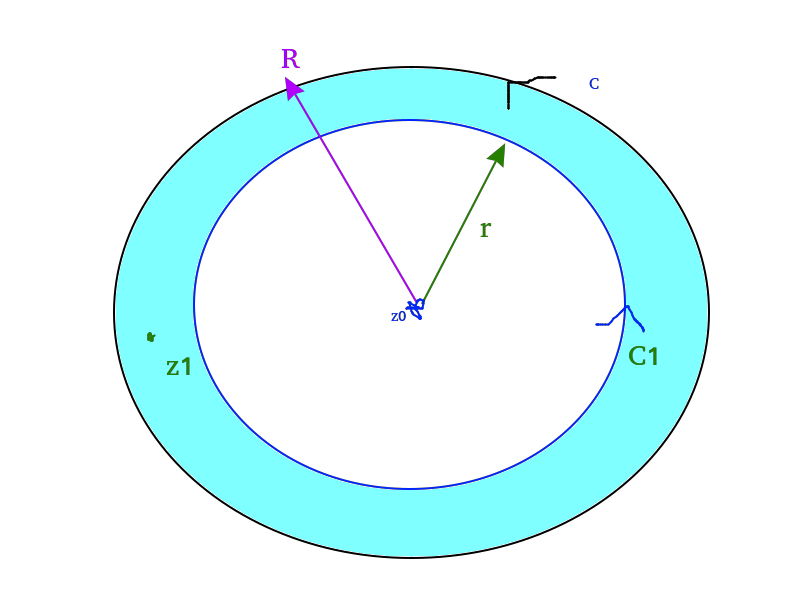
\includegraphics[width=0.7\linewidth]{riemann}
		\caption{Riemann's theorem proof graphics. In the blue annulus, $|f(z)|\leq M$.}
		\label{fig:riemann}
	\end{figure}
	Hence, by Cauchy, 
	\begin{align*}
	f(z_1) &= \frac{1}{2\pi}\int_C \frac{f(\zeta)}{\zeta - z_1} d\zeta - \frac{1}{2\pi i}\int_{C_1} \frac{f(\zeta)}{\zeta - z_1} d\zeta
	\end{align*}
	
	Note that the value of $f(z_1)$ is independent of $r$. We can say that:
	
	\begin{align*}
	\left|\frac{1}{2\pi i }\int \frac{f(\zeta)}{\zeta - z_1} d\zeta\right| \leq \frac{M2\pi r}{2\pi (|z_1-z_0|-r)}
	\end{align*}
	
	The RHS goes to zero as $r \to \infty$. And so:
	
	\begin{align*}
	f(z) = \frac{1}{2\pi i }\int_C \frac{f(\zeta)}{\zeta - z_1} d\zeta
	\end{align*}
	
	But the right hand side is analytic inside $C$. So define:
	\begin{align*}
	f(z_0) = \frac{1}{2\pi i }\int_C \frac{f(\zeta)}{\zeta - z_0} d\zeta
	\end{align*}
	
	Thus, the function $f(z)$ becomes analytic in the whole disk $|z-z_0|<R$. 
	
\end{theorem}

\begin{corollary}
If $f(z)$ has an isolated singularity at $z=0$ and is bounded in some neighborhood of $z_0$, then $\lim_{z \to z_0}f(z)$ exists. This singularity is a \textbf{removable singularity.}
\end{corollary}

\begin{ex}
An example of a removable singularity: let $f(z) = \frac{\sin z}{z}$ Since $\lim_{z \to z_0}f(z) = 1$, we can define $f(z)$ to be 1 at $z=0$ and the function becomes entire. 

\textbf{Note:} 

$$f(z) = 1 - \frac{z^2}{3!} + \frac{z^4}{5!} - ... $$
\end{ex}

\Def{Pole}{If $f(z)$ is defined in the deleted neighborhood of $z_0$, and a positive integer can be found such that:
$$\lim_{z \to z_0} (z-z_0)^n f(z) = A \neq \begin{cases}
0 \\ \infty 
\end{cases}$$

Then we say $f(z)$ has a pole of order $n$ at $z_0$. When $n=1$, the pole is simple.}

\begin{ex}
$f(z) = \frac{1}{z}$ has a simple pole at $z=0$. 
\end{ex}

\begin{theorem}
If $f(z)$ has an isolated singularity at $z = z_0$ and $f(z) \to \infty$ as $z \to z_0$, then $f(z)$ has a pole at $z=z_0$.

\textbf{Proof:}
If $f(z) \to \infty$ as $z \to z_0$, then $g(z) = 1/f(z)$ is bounded in some deleted neighborhood of $z_0$. By Riemann's theorem, $g(z)$ has a removable singularity at $z_0$ and we can write:

$$g(z) = \frac{1}{f(z)} = a_0 + a_1(z-z_0) + a_2(z-z_0)^2 + ..$$

It follows that $\lim_{z \to z_0}g(z) = a_0$

Now, the coefficients of $g(z)$ cannot all be zero. Suppose that $z_k$ is the first coefficient to be nonzero. Then, 

\begin{align*}
\frac{1}{f(z)(z-z_0)^k} = a_k + a_{k+1}(z-z_0) + a_{k+2}(z-z_0)^2
\end{align*}
Hence, $\lim_{z \to z_0} (z-z_0)^n f(z) = 1/a_k$ and $f(z)$ has a pole of the order $k$ at $z_0$.
\end{theorem}
\begin{corollary}
If $f(z)$ has a pole at $z=z_0$, then $f(z)$ may be expressed as $f(z) = \sum_{n=-k}^{\infty} b_n(z-z_0)^n$ where $k$ is the order of the pole. 
\end{corollary}

\Def{Essential Singularity}{An isolated singularity that is neither removable nor a pole is called an isolated essential singularity.}

\begin{theorem}
If $f(z)$ has an isolated essential singularity $z=z_0$, then $f(z)$ comes arbitrarily close to every complex value in each deleted neighborhood of $z_0$. 

\textbf{Proof:} Assume, that for some complex a, there is some $\epsilon>0$ such that $|f(z)-a|\leq \epsilon$ for all $z$ in $0 |z-z_0|<\delta$. 

Set $g(z) = \frac{1}{f(z)-a}$. Steps show how singularity must either be removable or pole. 

\end{theorem}
\begin{theorem}[Generalization of previous theorem, Picard]
In the neighborhood of isolated essential singularities, a function assumes each complex value, with one possible exception, infinitely often!
\end{theorem}

\begin{ex}
$f(z) = e^{1/z}$ has an isolated essential singularity at $z=0$ and never assumes a value of zero. Picard says that it must assume every other value in the neighborhood of the origin infinitely often.

Look for values of $z$ close to zero such that $e^{1/z}=i$. First, we note that $|e^{1/z}|=|i|=1$. This is only the case if the real part of $z= 0$. Now, set $z=iy$, $y\in\R$, then $e^{1/(iy)} = e^{i/y} = \cos(1/y) - i \sin (1/y) = i$. We see this is true when $1/y = -\pi/2 + 2 n \pi,\ n \in \mathbb{Z}$. 

Setting $z_n = \frac{1}{i(-\pi/2+2n\pi)}$, we have that $e^{1/z_n} = i$ for each $n$. Ovserve that there are infinitely many $z_n$ in the neighborhood of $z_0=0$. 
\end{ex}

\Def{Point at infinity singularity (functions)}{A function $f(z)$ has an isolated singularity at $z=\infty$ if $f(z)$ is analytic in the neighborhood $z=\infty$. Note that $f(z)$ is analytic for $|z|>R$ if and only if $f(\frac{1}{z})$is analytic for $\frac{1}{|z|}< \frac{1}{R}$ . Hence, $f(z)$ has an isolated singularity at $z=\infty$ if and only if $f(\frac{1}{z})$ has an isolated singularity at $z=0$. 

Moreover, we can say a singularity is removable or essential according to the singularity of $f(1/z)$ at $z=0$} 

\begin{ex}
	$f(z) = z^2+1$. This function has a pole of order 2 at $z=\infty$. This is true since $f(\frac{1}{z}) = \frac{1}{z^2}+1$ has a double pole at $z=0$. 
	
	$g(z) = e^z$ has an isolated essential singularity at $z=\infty$
\end{ex}

\subsection{Entire Functions}

\textbf{Note:} If $f(z) = \sum_{n=0}^k a_nz^n$ which is a polynomial of degree $k$, and as $z \to \infty$, the function blows up. If we look at 
$$f(\frac{1}{z}) = \frac{1}{z^k}\left(a_k \sum_{n=0}^{k-1} a_n z^{k+n}\right)$$

We see that since these powers are positive on the RHS, there is a pole of order $k$ at $z=0$. 

Hence, $f(z)$ has a pole of order $k$ at $z=\infty$. This is consistent with an earlier result. $f(z) \to \infty$ as $z \to \infty$. 

\textbf{Note: } A function $f(z)$ that has a pole of order k at $z= \infty$ if and only if 
$$\lim_{z\to\infty} \frac{f(z)}{z^k} = A \neq \begin{cases}
0 \\ \infty 
\end{cases}$$


Also by an earlier result, for entire functions, if the above condition is satisfied, then $f(z)$ is a polynomial of degree $k$. That is, transcendental entire functions must have essential singularities at the point at infinity. 

\Section{Laurent Series and Residues}
\subsection{Laurent Series}
Laurent series are a "generalization" of power series. We have seen that if $f(z)$ has a pole of order $k$ at $z=z_0$, then we find that $f(z)$ has a representation of the form $f(z) = \sum_{n=-k}^\infty a_n(z-z_0)^n$, $(a_{-k} \neq 0)$. 

This is valid in some deleted neighborhood about $z_0$. 

Next, consider the series:

\begin{align*}
f(z) = \sum_{m=-\infty}^{\infty} a_m(z-z_0)^m
\end{align*}


First note that 

\begin{align*}
\sum_{n=1}^\infty b_n(z-z_0)^{-n} & = \sum_{m=-\infty}^{-1} a_m (z-z_0)^m
\end{align*}

This represents a function $f_1(z)$ which is analytic for some $|z-z_0|>R_1$. This is because $\sum_{m=1}^\infty b_m(z-z_0)^{-m}$ is analytic for $|z-z_0|^{-1}<R = \frac{1}{R_1}$. 

Next, suppose $f_2(z) = \sum_{n=0}^\infty a_n(z-z_0)^n$ is analytic for $|z-z_0|>R_2$. Now we have broken up our function into circles bounded by $R_1, R_2$. So now we can say that if it so happens that $R_2>R_1$, then we get an annulus, and $f(z) = f_1(z) + f_2(z)$ in the annulus $R_1  < |z-z_0| < R_2$. 

\Def{Laurent Series}{
Suppose $f(z)$ is analytic in the annulus $R_1  < |z-z_0| < R_2$. 
The Laurent series of a function $f(z)$ is given by

\begin{align*}
f(z)=\sum _{n=-\infty }^{\infty }a_{n}(z-z_0)^{n}
\end{align*}
where $a_n$ and $z_0$ are constants, with an defined by a line integral that generalizes Cauchy's integral formula:

\begin{align*}
a_{n}={\frac {1}{2\pi i}}\oint _{C }{\frac {f(\zeta)}{(\zeta-z_0)^{n+1}}}\,d\zeta
\end{align*}

$C$ is any simple closed contour inside of the annulus that makes a complete counterclockwise revolution about $z_0$. 


\textbf{Proof:} Much like Taylor's theorem. 

$$f(z) = {\frac {1}{2\pi i}}\oint _{R_1  = |z-z_0| }{\frac {f(\zeta)}{(\zeta-z_0)^{n+1}}}\,d\zeta - {\frac {1}{2\pi i}}\oint _{R_2  = |z-z_0| }{\frac {f(\zeta)}{(\zeta-z_0)^{n+1}}}\,d\zeta $$
}

\textbf{Note:} A series of positive powers of $z-z_0$ converges inside $R_2  = |z-z_0|$. It is called the \textit{analytic part}. The series of negative powers converges outside $R_1  = |z-z_0|$ and is called the \textit{principal part}. Both are analytic, just have funny names. 

\begin{remark}
If $R_1 = 0$, the point $z_0$ is an isolated singularity. There are three cases:
\begin{enumerate}
	\item The principal part vanishes if and only if the singularity is removable.
	\item The principal part has finitely many terms if and only if the singularity at $z_0$ is a pole.
	\item If it is neither of the other cases, the principal part has an infinite number of terms if and only if the singularity at $z_0$ is an essential singularity. 
\end{enumerate}
\end{remark}

\textbf{Note:} The Laurent series representation is unique. 


\begin{ex}[Laurent Series expansion]
	Let $f(z) = \frac{1}{z^2 +1} = \frac{1}{(z-i)(z+i)}$. Then, $f$ has simple poles at $z=\pm i$. We note that $f(z)$ is analytic for $0 < |z-i| < 2$. This is an annulus with outer radius almost 2 expanded around $z=i$. And we can expand about $z=i$:
	
	\begin{align*}
	\frac{1}{z+i} &= \frac{1}{2i[1 + \frac{z-i}{2i}]} \\
	&= \frac{1}{2i}\sum_{n=0}^\infty (-1)^n \left(\frac{z-i}{2i}\right)^n
	\end{align*}
	
	Hence:
	\begin{align*}
	f(z) &= \frac{1}{2i(z-i)} \sum_{n=0}^\infty \left(\frac{-1}{2i}\right)^n (z-i)^n,\  \forall z \text{ s.t. } 0 < |z-i| < 2 \\ 
	&= \sum_{n=-1}^\infty \left(\frac{i}{2}\right)^{n+2} (z-i)^n,\ \forall z \text{ s.t. }0 < |z-i| < 2
	\end{align*}
	This converges for $0 < |z-i| < 2$. We can also expand about $z=-i$ to get the Laurent series:
	\begin{align*}
	f(z) = - \sum_{n=-1}^\infty \left(\frac{-i}{2}\right)^{n+2} (z+i)^n,\ \forall z \text{ s.t. }0 < |z+i| < 2
	\end{align*} 
\end{ex}


\subsection{Residues}
\Def{Residue}{The coefficient $a_{-1}$ is a special case, or the integral of the function in the Laurent series. It is called the residue of $f(z)$ at $z=z_0$. It is such that 

\begin{align*}
\frac{1}{2\pi i}\int_C f(\zeta) d\zeta = a_{-1}
\end{align*}

}

\begin{theorem}[Residue Theorem]
Suppose that $f(z)$ is analytic inside and on a simple closed contour $C$ except for isolated singularities at $z_1, z_2,..,z_n$ inside $C$. Let the residues at these points be $\alpha_1, \alpha_2,..,\alpha_n$ respectively. Then we can compute the following:


\begin{align*}
\int_C f(z) dz = 2 \pi i \sum_{i=1}^n \alpha_i
\end{align*}

\textbf{Proof:}

\begin{figure}[H]
	\centering
	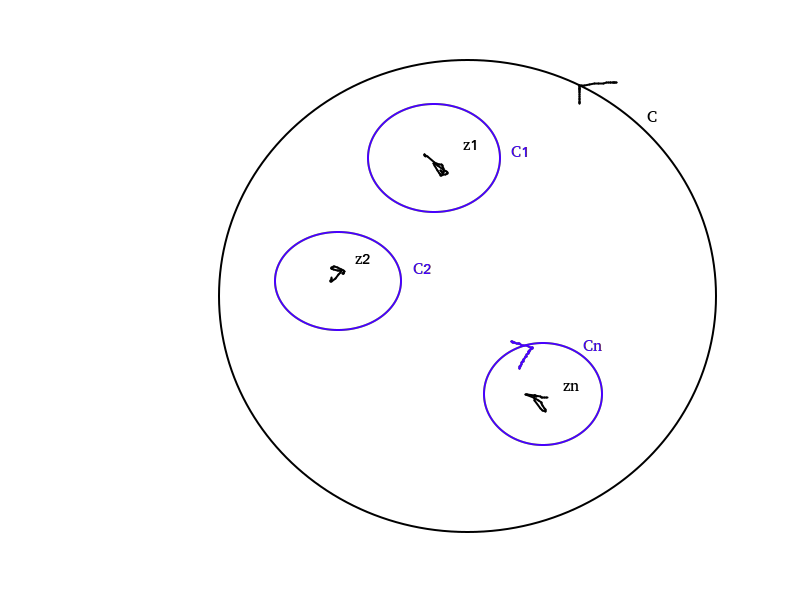
\includegraphics[width=0.5\linewidth]{cnn}
	\caption{Contours for proof}
	\label{fig:cnn}
\end{figure}


By the Cauchy Integral Formula, 

\begin{align*}
\int_C f(z) dz = \int_{C_1} f(z) dz + \int_{C_2} f(z) dz + .. + \int_{C_n} f(z) dz
\end{align*}

We note the terms are residues, so 

\begin{align*}
\int_C f(z) dz = \sum_{k=1}^n \alpha_k 
\end{align*}


\end{theorem}

\textbf{Note:} The Cauchy Integral formula is the special case of the residue theorem.

\begin{enumerate}
	\item Suppose $f(z)$ is analytic inside of a simple closed contour $C$ containing $z_0$. Then :
	
	$$g(z) = \frac{f(z)}{z-z_0}$$
	
	$g(z)$ has a simple pole at $z=z_0$ provided $f(z)$ is analytic and $f(z_0) \neq 0$. The residue of $g(z)$ at $z_0$ is:
	
	$$\lim_{z \to z_0}(z-z_0)g(z) = f(z_0)$$
	
	Therefore, $\int_C g(z) dz = 2 \pi i f(z_0)$. Thus concludes the Cauchy Integral Formula. 
\end{enumerate}

% 10/16
\textbf{Note:} Suppose $f$ has a pole of order $k$ at $z_0$. To find the residue $a_{-1}$ in terms of $f$, consider:

$$(z-z_0)^k f(z) = a_{-k}+...+a_{-1}(z-z_0)^{k-1}+ g(z)(z-z_0)^k$$

where $g$ is analytic. We differentiate this $k-1$ times and evaluating $z=z_0$, we find that:

$$a_{-1} = \frac{1}{(k-1)!} \lim_{z \to z_0} \dv{{}^{k-1}}{z^{k-1}} (z-z_0)^k f(z)$$

\begin{ex}
Suppose:
$$\int_C \frac{z^4-z^3+17z+2}{(z-1)^3}dz$$. 

\begin{figure}[H]
	\centering
	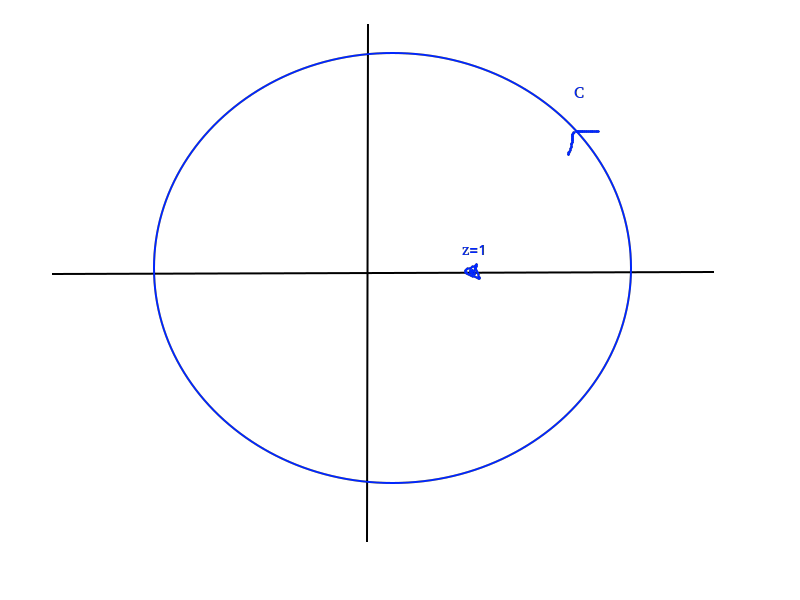
\includegraphics[width=0.5\linewidth]{contour_Ex}
	\caption{Contour in example.}
	\label{fig:contourex}
\end{figure}

We would like to find the residue of this. 

\textbf{Method 1:}

Set $f(z) =  \frac{z^4-z^3+17z+2}{(z-1)^3}$. Then:
\begin{align*}
a_{-1} &= \frac{1}{2!} \lim_{z\to1} \dv{^2}{z^2} (z-1)^3 f(z) \\ 
&= 3
\end{align*}

By the residue theorem:

$$\int_C f(z) dz = 2 \pi i  a_{-1} = 6 \pi i$$


\textbf{Method 2:}

Let $g(z) =  z^4-z^3+17z+2$. By the Cauchy Integral Formula:

$$g''(z) = \frac{2!}{2\pi i }\int_C \frac{g(z)}{(z-1)^3}dz$$
\end{ex}

\begin{theorem}
Let $g(z)$ and $h(z)$ be analytic at $z=z_0$, such that $g(z_0) \neq 0,\ h(z_0) \neq 0$ and $h'(z_0) = 0$. This implies that $f(z) = g(z)/h(z)$ has a simple pole with residue $g(z_0)/h'(z_0)$ at $z=z_0$. 

Note that since $g$, $h$ are analytic at $z=z_0$, they have Taylor series expansions of the form:

$$g(z) = \sum_{n=0}^\infty \gamma_n (z-z_0)^n $$
$$h(z) = \sum_{n=0}^\infty \delta_n (z-z_0)^n $$


By hypothesis, we have that $\gamma_0 \neq 0$. But $\delta_0 = 0$, and $g(z_0) = \gamma_0$ and $h'(z_0) = \delta_1$. Therefore, 

\begin{align*}
f(z) = \frac{g(z)}{h(z)} & = \frac{\sum\gamma_n (z-z_0)^n}{\sum\delta_n (z-z_0)^n} \\ 
& = \frac{\gamma_0}{\delta_1 (z-z_0)} \frac{1 + \sum\frac{\gamma_n}{\gamma_0} (z-z_0)^n}{\sum\frac{\delta_n}{\delta_1} (z-z_0)^n} 
\end{align*}

Then $f(z)$ has a simple pole at $z=z_0$, which gives us the result that 

\begin{align*}
a_{-1} &= \lim_{z \to z_0}(z-z_0) f(z) \\ 
& = \frac{\gamma_0}{\delta_1}
\end{align*}
\end{theorem}

\subsection{Non-isolated Singularities }
So far, everything we have done only applies to \textit{isolated singularities}. What about non-isolated singularities? Consider the function:

$$f(z) = \frac{1}{\sin(1/z)}$$

This has a singularity at $z=0$ since $\lim_{z\to0} f(z)$ does not exist. Furthermore, the points $z_n = \frac{1}{n\pi}$ are also singularities of $f(z)$. Since $z_n \to 0$ as $n \to \infty$, each deleted neighborhood of the origin contains a singularity of $f(z)$. 


Consider an additional example of a branch point. Let $f(z) = \log z$. This has a branch point at $z=0$. From this, we can define a \textit{branch} of $f$ such as the \textit{principal branch}, $\text{Log } z$, which is the single-valued in the cut plane (branch cut on the negative real axis.) If we exclude the origin, is $\text{Log }z$ analytic? Is it analytic in a deleted neighborhood around the branch point? No, because it is discontinuous on the branch cut (negative real axis). The origin is \textit{not} an isolated singularity. A branch point is \textit{never} an isolated singularity.

\Section{Real Integrals}
\subsection{Evaluation of Real Integrals}
\begin{ex}
Evaluate 
\begin{align*}
\int_0^\infty \frac{\sin x}{x} dx 
\end{align*}
This is kind of hard, so let's just exploit the $e^{iz} = \sin z + i \cos z$. 
Consider $\int_C \frac{e^{iz}}{z} dz$, where $C$ is a semicircular annulus enclosing the positive imaginary plane excluding the origin. It has an inner radius of $\epsilon$ and outer radius of $R$, so we can characterize it with $z=re^{i\theta}$, where $r \in [\epsilon, R]$ and $\theta \in [0, \pi]$ This has no singularities, so it equals zero. 

Also:
\begin{align*}
\int_C \frac{e^{iz}}{z} dz & = 0 \text{ (no singularities, so zero)}\\ 
&= \int_{\epsilon}^R \frac{e^{ix}}{x}dx + \int_0^\pi \frac{e^{iRe^{i\theta}}}{Re^{i\theta}} iRe^{i\theta} d\theta + \int_{+R}^{+\epsilon}\frac{e^{-ix}}{x}dx + \int_{\pi}^{0} ie^{i\epsilon i e^{i\theta}} d\theta \\ 
&= \int_{\epsilon}^{R} \frac{e^{ix}-e^{-ix}}{x}dx + i \int_{0}^{\pi} e^{iRe^{i\theta}} d\theta - i \int_{0}^{\pi}e^{i\epsilon i e^{i\theta}} d\theta \\ 
&= 2 i \int_{\epsilon}^{R} \frac{\sin x}{x}dx + i \int_{0}^{\pi} e^{iRe^{i\theta}} d\theta - i \int_{0}^{\pi}e^{i\epsilon i e^{i\theta}} d\theta \\ 
\end{align*}

Now consider that:
\begin{align*}
\left|\int_{0}^\pi e^{iRe^{i\theta}} d\theta \right| &\leq \int_{0}^\pi \left|e^{iR \cos \theta - R \sin \theta } \right|d\theta \\ 
& = \int_{0}^\pi e^{-R\sin\theta} d\theta  \\ 
& = 2 \int_{0}^{\pi/2} e^{-R\sin\theta} d\theta \text{ (integral of halves are equal, so only need to do 2*half integral)}\\ 
& \leq  2 \int_{0}^{\pi/2} e^{-\frac{2R}{\pi}\theta} d\theta \text{ (linear function vs sine function)} \\ 
& = \frac{\pi }{R}(1-e^{-R}) 
\end{align*}

This is true since $|e^{iR \cos \theta}| = 1$. Also $\frac{\pi }{R}(1-e^{-R}) \to 0$ as $R \to \infty$.

Taking the limit as $R \to \infty$ for our original problem, we get that:

\begin{align*}
\int_0^\infty \frac{\sin x}{x} dx  &= \frac{1}{2} \int_{0}^{\pi} e^{i \epsilon e^{i \theta }} d\theta 
\end{align*}

As $\epsilon \to \infty$ , $\int_{0}^{\pi} e^{i \epsilon e^{i \theta }} d\theta = \pi$. In conclusion, we get that:
\begin{align*}
\int_0^\infty \frac{\sin x}{x} dx  &= \frac{pi}{2}
\end{align*}
\end{ex}

\begin{ex}
Consider with $a,b \in \R $ and $a<|b|$, 
\begin{align*}
\int_0^{2\pi} \frac{1}{a+b \cos \theta} d\theta
\end{align*}

We set $z=e^{i\theta}$ and let $C$ be the unit circle. Thus:

\begin{align*}
\int_0^{2\pi} \frac{1}{a+b \cos \theta} d\theta &= \int_C \frac{1}{iz[a+\frac{b}{2} (z+\frac{1}{z})]} d\theta
\end{align*}


TODO

We can find the residue at $z$: 
\begin{align*}
\lim_{z \to z_1} (z-z_1) f(z) = \frac{b}{2\sqrt{a^2-b^2}}
\end{align*}

Hence, by the residue theorem, 

\begin{align*}
\int_0^{2\pi} \frac{1}{a+b \cos \theta} d\theta &= \frac{2\pi i b}{2\sqrt{a^2-b^2}} \left(\frac{2}{bi}\right) \\ 
&= \frac{2\pi }{\sqrt{a^2-b^2}} 
\end{align*}


\end{ex}

\begin{ex}
Find the value of:
$$\int_0^\infty \sin u^2 du$$

\textbf{Solution:}
We note that $F(x) = \int_0^x \sin u^2 du$. 

Let $f(z) = e^{iz^2}$ and $C$ be a contour that is a sector of a circle with an angle 0 to $pi/4$ and radius R. So by Cauchy's theorem, since there are no singularities in the contour:


\begin{figure}[H]
	\centering
	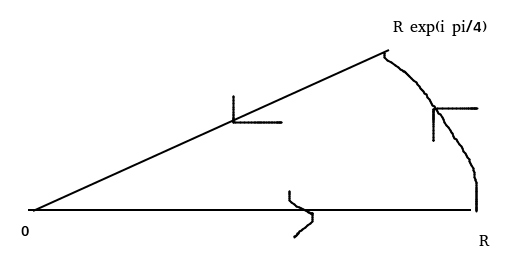
\includegraphics[width=0.4\linewidth]{sector_contour}
	\caption{Contour for Example}
	\label{fig:sectorcontour}
\end{figure}

$$\int_C e^{iz^2} dz=0$$



We want to relate this to our original integral. We can break up all parts of our contours
\begin{align*}
\int_0^R e^{ix^2} dx + \int_0^{\pi/4} e^{i R^2 e^{2i\theta}} d\theta + \int_R^0 e^{i(te^{i\pi/4})^2} e^{i\pi/4} dt = 0 
\end{align*}

Since we've chosen the angle $\pi/4$, we can have the nice form of the gaussian integral on the RHS: 

\begin{align*}
\int_0^R e^{ix^2} dx + \int_0^{\pi/4} e^{i R^2 e^{2i\theta}} d\theta = e^{i\pi/4}  \int_0^R e^{-t^2} dt
\end{align*}

We note te RHS can also be computed using contour integration. Looking at the second term, utilizing $e^{i2\theta} = \cos 2\ theta + i \sin 2 \theta $:

\begin{align*}
\left| \int_0^{\pi/4} e^{i R^2 e^{2i\theta}} d\theta \right| &\leq R \int_0^{\pi/4} e^{-R^2 \sin 2 \theta } d\theta \\
&= \frac{R}{2} \int_{0}^{\pi/2} e^{-R^2 \sin \theta } d\theta \text{   (change of variables)}\\ 
& \leq \frac{R}{2} \int_{0}^{\pi/2} e^{-R^2 \theta /\pi^2} d\theta \\ 
& = \frac{R}{2} \frac{\pi}{2R^2} (1-e^{-R^2}) \\ 
& = \frac{\pi}{4R}(1-e^{-R^2})
\end{align*}

Finally, if we take the limit, we get zero: $\lim_{R\to \infty } \frac{\pi}{4R}(1-e^{-R^2}) = 0$.


Now considering the integral again:

\begin{align*}
\int_0^R e^{ix^2} dx = e^{i\pi/4}  \int_0^R e^{-t^2} dt
\end{align*}

However, we note that $\int_0^\infty e^{-t^2} dt = \sqrt{\pi}/2$, which is a \textit{Gaussian Integral.}
And so:

\begin{align*}
\int_{0}^{\infty} (\cos x^2 + i \sin x^2  )dx = \frac{1}{\sqrt{2}} (1+i)\sqrt{\pi}/2
\end{align*}

Taking just the real parts or imaginary parts to get the integrals of $\sin x^2$ or $\cos x^2$. 

\textbf{Note:} We can also compute a \textit{gaussian integral} using contour integration. Let $a=\sqrt{\pi i} = (1+i) \sqrt{\pi/2}$ and:

$$g(z) = \frac{e^{-z^2}}{1+e^{-2az}}$$

The contour we are integrating over is: 
\begin{figure}[H]
	\centering
	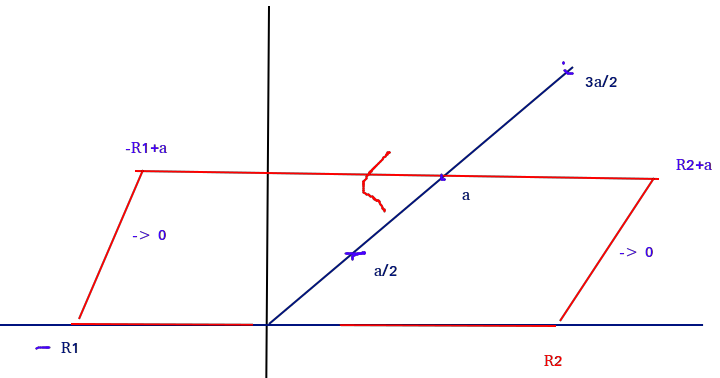
\includegraphics[width=0.7\linewidth]{box_c}
	\caption{Contour for Example. The Right and left sides go to zero, so subtract top from bottom to get the value of the integral over the red contour.}
	\label{fig:boxc}
\end{figure}

\begin{align*}
\int_C g(z) dz = 2\pi i \Res[g(z=a/2)]
\end{align*}
\end{ex}

\begin{ex}
Consider evaluating:
\begin{align*}
\int_0^\infty \frac{x^{\lambda-1 }}{1+x} dx,\ \lambda \in (0,1)
\end{align*}

Consider $f(z) = \frac{z^{\lambda-1}}{1+z}$, with branch cut $0 < \arg z < 2 \pi $. There is  a branch cut from 0 to $\infty$, so let us take the branch cut to the positive reals, such that we do not intersect our pole at $z=-1:$

\begin{figure}[H]
\centering
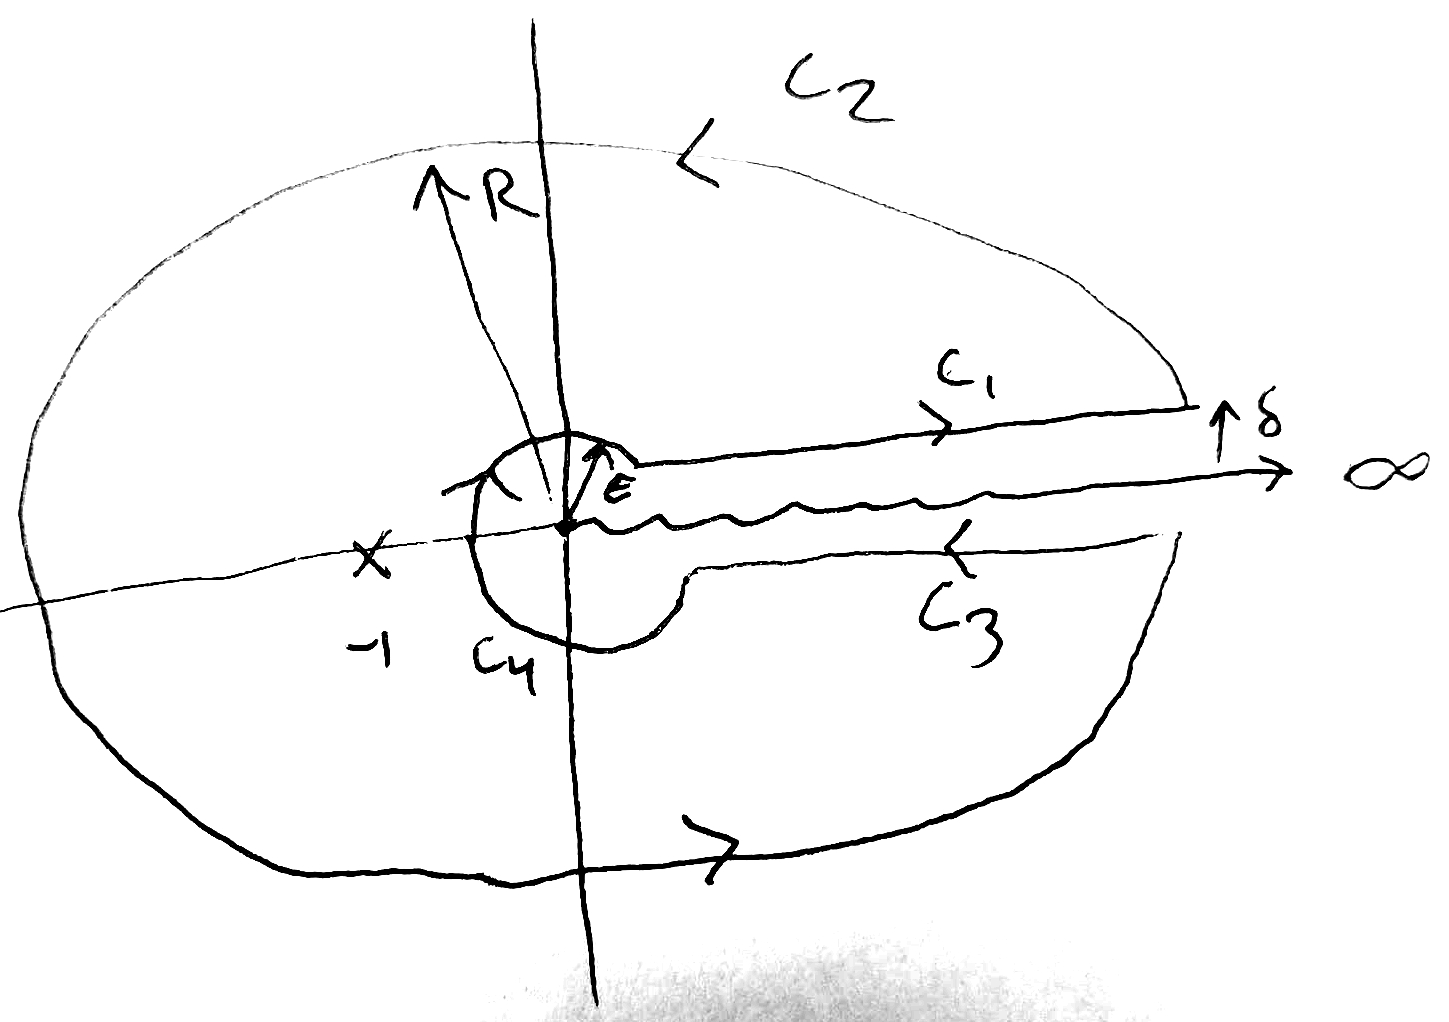
\includegraphics[width=0.7\linewidth]{mycontour}
\caption{}
\label{fig:branchc}
\end{figure}

$f(z)$ has a simple pole at $z=-1$ with a residue:

\begin{align*}
\Res[f, -1] = \lim_{z \to -1} (1+z)f(z) = e^{\pi i (\lambda - 1)} 
\end{align*}

We pick the contour which is the whole plane excluding the branch cut $C = C_1 + C_2 + C_3 + C_4$. By the residue theorem:

\begin{align*}
\int_C \frac{z^{\lambda-1}}{1+z} dx = 2 \pi i e^{i \pi (\lambda-1)} \\ 
 = \int_{C_1} + \int_{C_2} + \int_{C_3} + \int_{C_4}
\end{align*}

Considering the $C_1$ integral, let $\delta, \epsilon \to 0$, and $R \to \infty$. 

\begin{align*}
\int_{C_1}\frac{z^{\lambda-1}}{1+z} dx &= \int_{C_1} \frac{(x+i\delta)^{\lambda-1}}{1+(x+i\delta)} dx \\ 
& = \int_\epsilon^R \frac{x^{\lambda-1 }}{1+x} dx \text{ (as $\delta$ to 0)} \\ 
\end{align*}

Also we note that:
\begin{align*}
\int_{C_1}\frac{z^{\lambda-1}}{1+z} dx &= \int_R^\epsilon \frac{(x-i\delta)^{\lambda-1}}{1+(x-i\delta)} dx \\ 
& = \int_R^\epsilon \frac{e^{i2\pi(\lambda-1)}}{1+x} dx \text{ (as $\delta$ to 0)} \\ 
& = -e^{i2\pi\lambda} \int_R^\epsilon \frac{x^{(\lambda-1)}}{1+x} dx \text{ (as $\delta$ to 0)} 
\end{align*}


We still have to deal with the other integrals. Let $z=Re^{i\theta}$

\begin{align*}
\left| \int_{C_2} \frac{z^{\lambda-1}}{1+z} dz\right| &= \int_0^{2\pi} \frac{(Re^{i\theta})^{\lambda-1} i Re^{i\theta}}{1 + Re^{i\theta}} d\theta \\ 
&\leq  R^\lambda \left| \frac{1}{R-1}\right| \\
& = \frac{2\pi R^\lambda}{R-1}
\end{align*}

As we take $R \to \infty$:
\begin{align*}
\lim_{R\to \infty } \left| \int_{C_2} \frac{z^{\lambda-1}}{1+z} dz\right| &\leq  0
\end{align*}


Finally, we look at $C_4$:

\begin{align*}
\left| \int_{C_4} \frac{z^{\lambda-1}}{1+z} dz\right| &= \left|\int_0^{2\pi } \frac{(\epsilon e^{i \theta(\lambda -1)})\epsilon e^{i \theta}}{1 + \epsilon e^{i \theta}} d\theta \right| \\ 
& \leq \frac{\epsilon^\lambda}{1-\epsilon} \int_{0}^{2\pi }d\theta = 2 \pi \frac{\epsilon^\lambda}{1-\epsilon}
\end{align*}

This goes to 0 as $\epsilon \to 0$. Now:

\begin{align*}
\int_C \frac{z^{\lambda-1}}{1+z} dx = 2 \pi i e^{i \pi (\lambda-1)} \\ 
= \int_{C_1} +\int_{C_3} + \int_{C_2} +  \int_{C_4} \\ 
=  (1-e^{i2\pi\lambda}) \int_0^\infty \frac{x^{(\lambda-1)}}{1+x} dx+ 0 + 0
\end{align*}

Finally, we see that: 
\begin{align*}
\int_0^\infty \frac{x^{(\lambda-1)}}{1+x} dx = \frac{2\pi i e^{i \pi \lambda }}{e^{i2 \pi \lambda } - 1} \\ 
= \pi \left(\frac{2i}{e^{i \pi \lambda } - e^{-i \pi \lambda }}\right)
= \frac{\pi}{\sin \pi \lambda }
\end{align*}

\end{ex}

These ideas, while useful for evaluating real integrals, can also be used to generate series representations for functions with poles. Or, we can do representations for functions with zeros. If a function has zeros which converges to a limit point, the function must be a zero function. 

However, if the series of zeros do not converge, this identity theorem does not apply. We can use the Weirstrass Factorization theorem to generate an expression for the function in terms of the values of the zeros. The expansion will be dependent on the zeros of the function:

$$\sin z = \sum_{n=-\infty}^{\infty}(f(zeros))$$

\subsection{Special Contour Integrals}
\begin{lemma}[Jordan's]
Let $f(z) = e^{iaz}g(z),\ a>0$ be a continuous function defined on a \textbf{semi-circular} counter-clockwise contour in the upper half plane centered around the origin:

$$C_r = \{Re^{i\theta}| \theta \in [0, \pi]\}$$

Then we can say that:

\begin{align*}
\left|\int_{C_R}f(z) dz\right| \leq \frac{\pi}{a} M_R
\end{align*}

where $M_R := \max_{\theta \in [0,\pi]}|g(Re^{i\theta})|$ 
\end{lemma}

Alternative Jordan's lemma:

If the only singularities in $g(z)$ are poles, $a>0$, and $g(z) \to 0$ as $R \to \infty$, then 

$$\lim_{R \to \infty} \int_{C_R}e^{iaz}g(z) dz = 0$$

\begin{lemma}[Indentation Lemma]
Let $f$ have a simple pole at $a$ with a residue $\Res[f;a]$. Then given an upper half clockwise semi-circular contour around the pole $C_\epsilon$, the resulting contour is:

\begin{align*}
\lim_{\epsilon\to0} \int_{C_\epsilon} f(z) dz = -\Res[f;a]\pi i
\end{align*}
\end{lemma}

% 10-30

\section{Special Functions}
\subsection{Gamma Functions}
\textbf{Note:}
\begin{align*}
e^{-t} = \lim_{n\to\infty}(1-\frac{t}{n})^n
\end{align*}

Let us define a Gamma function as:

\begin{align*}
\Gamma(z;n) := \int_{0}^{n} (1-\frac{t}{n})^n t^{z-1} dt  
\end{align*}

Then:
\begin{align*}
\lim_{n\to\infty} \Gamma(z;n) = \Gamma(z)
\end{align*}

Now, let $t = m \tau$, $t^{z-1}dt = n^z \tau^{z-1} d\tau$. Then:

\begin{align*}
\Gamma(z;n) = n^z \int_{0}^{1} (1-\tau)^n \tau^{z-1} d\tau
\end{align*}

By I.B.P.:


\begin{align*}
\Gamma(z;n) &= n^z \left[ \frac{1}{z} \left((1-\tau)^n \tau^{z}\right)\right]_0^1 + \frac{n}{z}\int_{0}^{1} (1-\tau)^{n-1} \tau^{z} d\tau \\ 
&= n^z \left(\frac{n}{z}\int_{0}^{1} (1-\tau)^{n-1} \tau^{z} d\tau\right) \\
&= n^z \left(\frac{n}{z} \frac{n-1}{z+1}\int_{0}^{1} (1-\tau)^{n-2} \tau^{z+1} d\tau\right) \\
&...\\
&= \frac{n(n-1)...(2)(1)}{z(z+1)...(z+n-1)} n^z \int_{0}^{1} \tau^{z+n-1} d\tau 
\end{align*}

We can then conclude that $\Gamma(z)$ converges on:

\begin{align}\label{eq:gamman}
\Gamma(z) &= \lim_{n\to\infty} \frac{n! n^z}{z(z+1)...(z+n-1)} \\ 
 &= \lim_{n\to\infty} \frac{(n-1)! (n-1)^z}{(z)_n} 
\end{align}

\textbf{Note:}
\begin{align*}
\Gamma(z) &= \lim_{n\to\infty} \left(\frac{n-1}{n} \right)^z   \frac{(n-1)! (n)^z}{(z)_m} \\
&= \lim_{n\to\infty}  \frac{(n-1)! (n)^z}{(z)_n} 
\end{align*}

Recall that $(z)_n = \frac{\Gamma(z+n)}{\Gamma(z)}$, And thus with some algebraic manipulation:

\begin{align*}
\Gamma(z) &= \lim_{n\to\infty}\frac{(n-1)!n^z}{\Gamma(z+n)}\Gamma(z) \\ 
1 &= \lim_{n\to\infty}\frac{(n-1)!n^z}{\Gamma(z+n)}
\end{align*}

Now we see:

\begin{align*}
\Gamma(z) &= \lim_{n\to\infty} \frac{(n)! (n+1)^z}{(z)_{n+1}} \\ 
 &= \frac{1}{z} \lim_{n\to\infty} \frac{(n)! (n+1)^z}{(z+1)...(z+n)} \\ 
  &= \frac{1}{z} \lim_{n\to\infty} \frac{((n+1)^z}{(1+z)(1+z/2)...(1+z/n)} \\ 
  &= \frac{1}{z} \prod_{k=1}^{\infty} \frac{(1+\frac{1}{k})^z}{(1+\frac{z}{k})}
\end{align*}

This is shown by \textbf{Gauss}. This infinite product (take the log) converges and therefore represents an analytic function for $z \neq 0, -1, -2,...$. The function also provides analytic continuation into $\Re{z} \leq 0$. 

\Def{Gamma Function}{
A Gamma function is a special function of the form:
\begin{align*}
\Gamma (z)=\int_{0}^{\infty}x^{z-1}e^{-x}\,dx
\end{align*}

If $z$ is complex with positive real part, then the integral converges absolutely, and $\Gamma(n) = (n-1)!$ for all positive integer $n$.

This formulation allows us to extend the idea of factorials to the complex numbers.
}

\Def{Euler-Mascheroni Constant}{
Let $s_n = \sum_{k=1}^n \frac{1}{k}$. This diverges as $n\to\infty$. However, 

\begin{align*}
\lim_{n\to\infty}(s_n - \log n) = \gamma = 0.5772...
\end{align*} 

We define the Euler-Mascheroni Constant as $\gamma$. 
We can also define the constant $\gamma$ as:

\begin{align*}
\gamma =  \int_0^\infty e^{-t} \left[\frac{1}{1-e^{-t}}-t\right]dt
\end{align*}
}

Now, from Equation \ref{eq:gamman}, we can see that:

\begin{align*}
\frac{1}{\Gamma(n)}  &= z \lim_{n\to\infty} m^{-z}\frac{(z+1)...(z+n-1)}{m!} \\ 
& = z \lim_{n\to\infty} (1+\frac{z}{1}) (1+\frac{z}{2}) ... (1+\frac{z}{n}) e^{-z\log m} \\ 
&  = z \lim_{n\to\infty} \left[\prod_{k=1}^n (1+\frac{z}{k}) e^{-z/k}\right] e^{z(1 + \frac{1}{2} + ... + \frac{1}{m} - \log m )}
\end{align*}

We note that $1 + \frac{1}{2} + ... + \frac{1}{m} - \log m  \to \gamma$, so:
\begin{align*}
\frac{1}{\Gamma(n)}  = z e^{\gamma z} \lim_{n\to\infty} \left[\prod_{k=1}^n (1+\frac{z}{k}) \right]
\end{align*}

This is provided by Weirstrass. This provides a factorization of $1/\Gamma(z)$ which is entire, with first order zeros only with $\Gamma(z)$ that has poles $z = 0, -1, -2...$. We note that since $1/\Gamma(z)$ has no poles, $\Gamma(z)$ can have no zeros!

Now, recall that:

\begin{align*}
\sin \pi z = \pi z \prod_{n=1}^\infty (1-\frac{z^2}{n^2})
\end{align*}

On the other hand, we have shown that:

\begin{align*}
\sin \pi z &= \frac{\pi}{\Gamma(z) \Gamma(1-z)} \\ 
&= \frac{-\pi}{z \Gamma(z) \Gamma(-z)} \\ 
&= \frac{\pi z^2}{z} \prod_{k=1}^\infty (1+\frac{z}{n})(1-\frac{z}{n})
\end{align*}

\begin{theorem}[Contour Integral Representation (Hankel)]
Consider a contour $C$:
\begin{figure}[H]
	\centering
	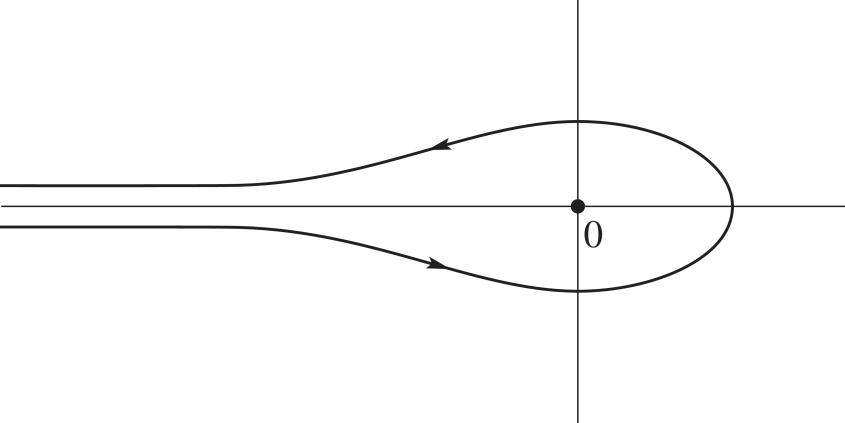
\includegraphics[width=0.7\linewidth]{hankel_contour}
	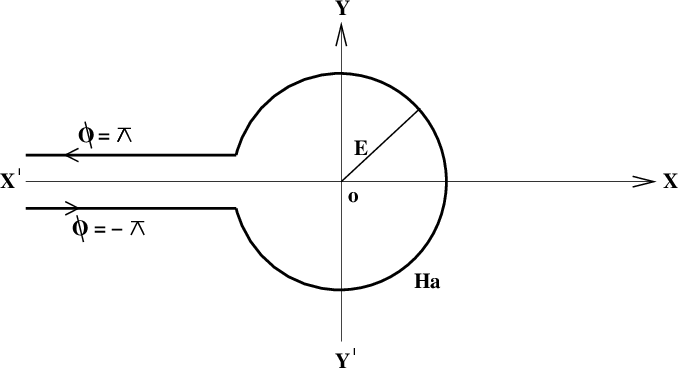
\includegraphics[width=0.7\linewidth]{hankel2}
	\caption{The Hankel contour in general, and then parameterized by a radius E or $\epsilon$. Call the circle contour $C_\epsilon$ or $\gamma_\epsilon$}
	\label{fig:hankelcontour}
\end{figure}



The contour lets us take a branch cut along the negative real axis. We let $\zeta = e^{-\pi r} = r$ on the top side, and $\zeta = e^{-i\pi}r = -r$


\begin{align*}
I &= \int_{C} e^{\zeta} \zeta^{-z} d\zeta \\ 
&= \int_{\infty}^{\epsilon} e^{-r} (re^{-i\pi})^{-z} e^{-i\pi}dr + \int_{C_\epsilon} f(\zeta) + \int_{\epsilon}^{\infty} e^{-r} (re^{i\pi})^{-z} e^{i\pi}dr
\end{align*}

As $\epsilon \to \infty$, $\int_{C_\epsilon} f(\zeta) \to 0$. Therefore:

\begin{align*}
I &= \int_{0}^{\infty} e^{-r} r^{-z} e^{i\pi z}dr  - \int_{0}^{\infty} e^{-r} r^{-z} e^{-\i pi z} dr \\ 
&= 2 i \sin \pi z  \int_{0}^{\infty} e^{-r} r^{-= z} e^{i\pi z}dr \\ 
&=  2 i \sin \pi z \Gamma(1-z) \\ 
&=  2 i \sin \pi z \frac{\Gamma(z)\Gamma(1-z)}{\Gamma(z)} \\ 
&= { 2 i \sin \pi z }{\Gamma(z) \sin \pi z} \\ 
&= { 2 i }{\Gamma(z) } 
\end{align*}

We then rearrange to get:

\begin{align*}
\frac{1}{\Gamma(z)} = \frac{1}{2\pi i } \int_{C} e^\zeta \zeta ^{-z} d\zeta 
\end{align*}

This form is valid for any value of $z$.
\end{theorem}

\subsection{Beta, Digamma, Riemann Zeta functions}

\Def{Beta Function}{
We define the Beta function as:
\begin{align*}
 \mathrm{B} (x,y)=\int _{0}^{1}t^{x-1}(1-t)^{y-1}\,dt
 = \frac{\Gamma(x)\Gamma(y)}{\Gamma(x+y)}
  \end{align*}
}

\Def{Digamma Function}{
The Digamma function (or Psi Function) is
\begin{align*}
\Psi (z) = \frac{\Gamma'(z)}{\Gamma(z)} = \dv{z} \left(\log \Gamma(z)\right)
\end{align*}

This is meneomorphic. It has simple poles at $z=0, -1, -2..$ The residue at each pole is $-1$. 

Now, recall

\begin{align*}
\log \Gamma(z) = -\log z - \gamma z - \sum_{k=1}^\infty \left[\log(1+\frac{z}{k}) - \frac{z}{k}\right]
\end{align*}

Then, 

\begin{align*}
\Psi(z) = - \frac{1}{z} - \gamma  - \sum_{k=1}^\infty \left[\frac{1}{k(1+\frac{z}{k})} - \frac{1}{k}\right]
\Psi(z) = - \frac{1}{z} - \gamma  + \sum_{k=1}^\infty \frac{z}{k(z+k)}
\end{align*}

This has simple poles at $z=0,-1,-2,...$. 

We note that $\Psi(1) = -\gamma$. \textit{("It's true by the way!"}) 

Additionally, recall that:
\begin{align*}
\Gamma(z+1) = z\Gamma(z) 
\end{align*}

By direct differentiation:
\begin{align*}
\frac{\Gamma'(z+1)}{\Gamma(z+1)} = \frac{\Gamma(z) + z \Gamma'(z)}{z \Gamma(z)} = \frac{1}{z} + \gamma(z)
\end{align*}

Then we can compute:
\begin{align*}
\Psi(1) = -\gamma\\
\Psi(2) = 1-\gamma \\ 
\Psi(3) = \frac{1}{2} + 1 - \gamma \\
...\\
\Psi(n+1) = \sum_{k=1}^{n} \frac{1}{k} - \gamma
\end{align*}

We see that $\Psi(n+1) \sim \log n$. 
}

\Def{Riemann Zeta Function}{
\begin{align*}
\zeta(s) = \sum_{n=0}^{\infty} \frac{1}{(1+n)^\zeta} \\ 
\frac{1}{\zeta(s)} = \prod_{p} (1-\frac{1}{p^s}),\ p \in \text{Primes}
\end{align*}

The poles of the Riemann Zeta Function are $-2, -4...$ 
}

\Section{ODEs}

\Section{Frobenius Theory}
% 11/15
\Section{Hypergeometric Equations}
\Def{Hypergeometric Equation}{
\begin{align}\label{eq:hg}
z(1-z)w''+[C-(A+B+1)z]w'-ABw=0
\end{align}

where $A,B,C$ are complex constants. 
}

\textbf{Note:} It is a $P$ Equation with $a=0, b=1, c\to \infty$, and its solution can be written as:

\begin{align*}
w = P\begin{bmatrix}[ccc|c]
0 & 1 & \infty& \\ 
0 & 0 & A & z\\ 
1-C & C-A-B & B &
\end{bmatrix} 
\end{align*}
\textbf{Note:} By suitable changes of dependent and independent variables, the general. P equation can be put in the above form for the hyper geometric equation. Therefore, solutions of the P equation can be expressed in terms of the sums of the hypergeometric equation.

\textbf{Note:} It can be shown that the hypergeometric series:

\begin{align*}
F(A,B,C;z) = 1+\frac{AB}{1C}z + \frac{A(A+1)B(B+1)}{(1)(2)C(C+1)}z^2+...
\end{align*}

Or as from Wikipedia:

\begin{align*}
{}_{2}F_{1}(a,b;c;z)=\sum _{n=0}^{\infty }{\frac {(a)_{n}(b)_{n}}{(c)_{n}}}{\frac {z^{n}}{n!}}.
\end{align*}

This series is convergent for $|z|<1$, and divergent $|z|>1$. This is a solution of the hypergeometric equation, or Equation \ref{eq:hg}.

We note that $C$ cannot be a negative integer.

We can use the transformation rules to get a second solution to the hypergeometric equation of the form:

\begin{align*}
z^{1-C} F(1+A-C, 1+B-C, 2-C; z)
\end{align*}

This solution, together with the previous solution of $F(A,B,C;z)$ provide 2 fundamental solutions of Equation \ref{eq:hg} in the vicinity of $z=0$. 

We note that expressions for the function F, which for $|z|>1$, may be obtained by contour integration. 

\subsection{Examples of ODE theory}
\Def{Legendre Polynomials}{
The following is the definition of Legendre polynomials using Rodriguez[french]'s formula:
\begin{align*}
P_n = \frac{1}{2^n n!} \dv{^n}{z^n} [(z^2-1)^n]
\end{align*}

Clearly, we see that:

\begin{align*}
P_0(z) &= 1\\
P_1(z) &= z\\
P_2(z)&= \frac{1}{2}(3z^2-1) 
\end{align*}

}

Since by Cauchy's formula's formula:

\begin{align*}
(z^2-1)^n = \frac{1}{2\pi i }\oint \frac{(\zeta^2-1)^n}{\zeta-z} d\zeta
\end{align*}

We take the contour integral representation (Schlafli's Integral):

\begin{align*}
P_n(z) = \frac{1}{2\pi i n!} \dv{^n}{z^n}\oint ... dz \\ 
= \frac{1}{2\pi i } \dv{^n}{z^n}\int_C \frac{(t^2-1)^n}{2^n(t-z)^{n+1}} dz
\end{align*}

Where $C$ is any contour that circles the point $t=z$ once in the counter clockwise direction.

\textbf{Note:}

\begin{align*}
\int_C \dv{t} \frac{(t^2-1)^{n+1}}{(t-z)^{n+2}} dt = 0
\end{align*}

This is because $\frac{(t^2-1)^{n+1}}{(t-z)^{n+2}}$ returns to its original value when $t$ circles $z$ once.

Carrying out differentiation and using Schlafli's integral  for $P_n(z)$, it can be seen that $P_n$ satisfies the \textbf{Legendre equation:}

\begin{align*}
(1-z^2)P_n'' - 2zPn' + n(n+1)P_n = 0
\end{align*}

This proof shoes that Schlafli's representation for $P_n$ still gives a solution to Legendre's equation for non-integer values of $n$ and provided that $C$ is still a close contour for which the expression  $\frac{(t^2-1)^{n+1}}{(t-z)^{n+2}}$ returns to its original value after a complete circuit.

One such contour is the following in Figure \ref{fig:legbp}.

\begin{figure}[H]
	\centering
	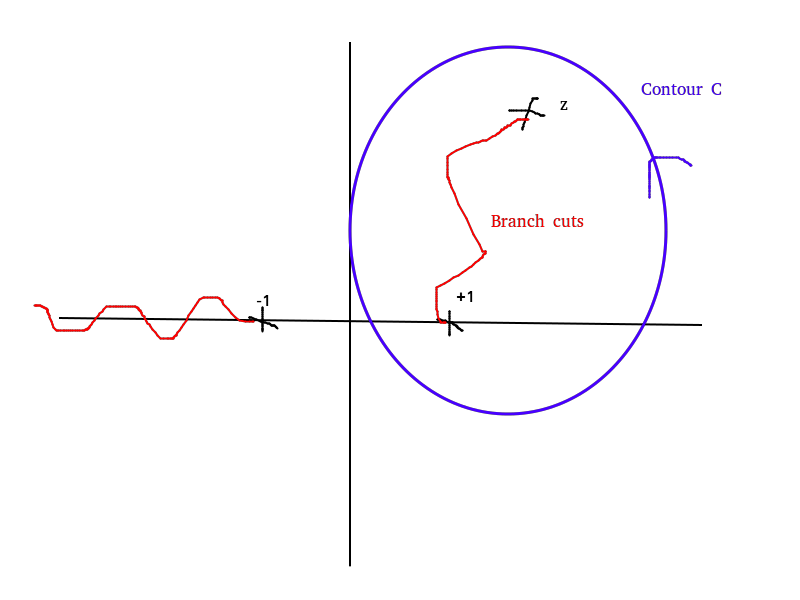
\includegraphics[width=0.7\linewidth]{leg_bp}
	\caption{There are poles at $-1, 1, z$, and branch point at infinity. So we must do the contour around it. Branch points are in red. This allows us to make a contour that surrounds $z$ }
	\label{fig:legbp}
\end{figure}

This choice of Branch cuts and contour $C$ still leads to solutions of the Legendre Equations when $n$ is not an integer. The solution is called a \textit{Legendre function of the first kind.} We not that we can use the the Schlafli form to derive a recursive equation:

\begin{align*}
(2n+1) P_n(z) = P_{n+1}'(z) + P_{n-1}'(z) \\ 
(z^2-1) P_n'(z) = nzP_n(z)-nP_{n+1}(z) \\ 
(n+1)P_{n+1}(z) - (2n+1)zP_n(z) + nP_{n+1}(z) = 0\\
nP_n(z) = zP_n'(z)-P_{n-1}'(z)
\end{align*}

\Def{Generating Function}{
A function $\phi(\zeta, z)$ such that 
\eq{\phi(\zeta, z) = P_0(z) + \zeta P_1(z) + \zeta^2 P_2(z) + ...}

for small values of $|\zeta|$ is a generating function.
}
Using the Schlafli representation:

\begin{align*}
\phi(\zeta,z) &= \frac{1}{2 \pi i} \int_C \left[\sum_{n=0}^\infty \frac{\zeta^n(t^2-1)^n}{2^n(t-z)^{n+1}}\right]dt \\ 
&= \frac{1}{2 \pi i} \int_C \frac{1}{t-z}\left[1 -  \frac{\zeta(t^2-1)^n}{2(t-z)}\right]^{-1}dt \\ 
&= \frac{1}{2 \pi i} \int_C \frac{dt}{t-z-\frac{\zeta(t^2-1)}{2}}
\end{align*}


The denominator vanishes for two values of $t$, but only 1 is inside $c$. The calculation of the residue gives the result:

\begin{align*}
\phi(\zeta,z)& = (1-2z \zeta + \zeta^2)^{-1/2} \\ 
&= 1 + \frac{1}{2} \left[\frac{-2z+2\zeta}{(1-2z\zeta + \zeta^2)^{3/2}} \right]_{\zeta=0}
\end{align*}

where the principal branch is taken. Then, for small $|\zeta|$, then 

\begin{align*}
\phi(\zeta,z) = P_0(z) + \zeta P_1(z) + \zeta^2 P_2(z)
\end{align*}

From this, we can check that $P_n(1)=1$:

\begin{align*}
P_n(-1)& = (-1)^n \\ 
P_n(-1) &= (-1)^n \\ 
P_n(-z) &= (-1)^nP_n(z) \\ 
P_{2n+1}(0) &= 0 
\end{align*}

\subsection{Laplace's Integrals}
If we use Schlafli's and let contour $C$ be a circle of radius $|z^2-1|^{1/2}$. Let us set $t=z + |z^2-1|^{1/2} e^{i\theta}$, where $\theta \in [-\pi, \pi]$. Then, 

\begin{align*}
P_n(z) &= \frac{1}{2^{n+1} \pi } \int_{-\pi}^\pi \left[\frac{z^2-1 + 2z(z^2-1)^{1/2} e^{i\theta} + (z^2-1)^{1/2} e^{i2\theta}}{(z^2-1)^{1/2} e^{i\theta}}\right]^n d\theta \\ 
&=\frac{1}{ \pi } \int_{0}^\pi [z +(z^2-1)^{1/2} \cos \theta ]^n d\theta 
\end{align*}

This is called \textbf{Laplace's first integral.}

\Def{Laplace's Second Integral}{
\begin{align*}
P_n(z) = \pm \frac{1}{\pi} \int_{0}^\pi \frac{d\theta}{ [z +(z^2-1)^{1/2} \cos \theta ]^n }
\end{align*}
}

\subsection{Legendre functions and their kinds}

%11-18
Consider again Legendre's equation:

\eq{(1-z^2)w'' - 2zw' + \nu(\nu +1)w = 0}
This function is a Legendre function of the first kind. THis equation has 3 regular singularities at $z=\pm1, \infty$ in the finite plane. its solutions are analytic, but not necessarily single valued except at $z=\pm 1$.

The indicial equation gives both roots $\rho = 0$. The branch points at $\pm 1$ are logarithmic. In the vicinity og he origin, the solution is analytic and we can look for expansions of the form:

\eq{w = a_0 + a_1 z + a_2z^2+...}

As we expand, we get two solutions, where $F$ is the hypergeometric equation:

\begin{align*}
w_1(z) &= 1-\frac{\nu(\nu+1)}{2!}z^2 + \frac{\nu (\nu-2) (\nu+1) (\nu+3)}{4!}z^4+... \\ 
&= F(-\frac{\nu}{2}, \frac{\nu+1}{2}, \frac{1}{2}; z^2)
\end{align*}

\begin{align*}
w_1(z) = zF(-\frac{1-\nu}{2}, \frac{\nu+2}{2}, \frac{3}{2}; z^2)
\end{align*}

These solutions are linearly independent. The general solution for $|z|<1$ of the form 

\eq{w = A w_1 + B w_2,\ A,B\in \C}

As we have seen, Schlafli's representation provides the analytic continuation of one solution. 

\textbf{Note:} at the point $z=1$, the integrand does not have a branch point. By taking derivatives of $P_\nu$ and evaluating the taylor expansion about $z=1$, we get 

\begin{align*}
P_\nu(z) = F(\nu+1, -\nu, 1; \frac{1-z}{2})
\end{align*}

This equation is analytic at $z=1$, but not necessarily analytic at $z=-1$.

Now let us consider \textbf{Legendre functions of the second kind}, with contour in Figure \ref{fig:leg2}:

\begin{align*}
Q_\nu(z) = \frac{1}{2i\sin \nu \pi } \int_C \frac{(t^2-1)^\nu}{2^\nu (z-t)^{\nu+1}}dt 
\end{align*}

\begin{figure}[H]
	\centering
	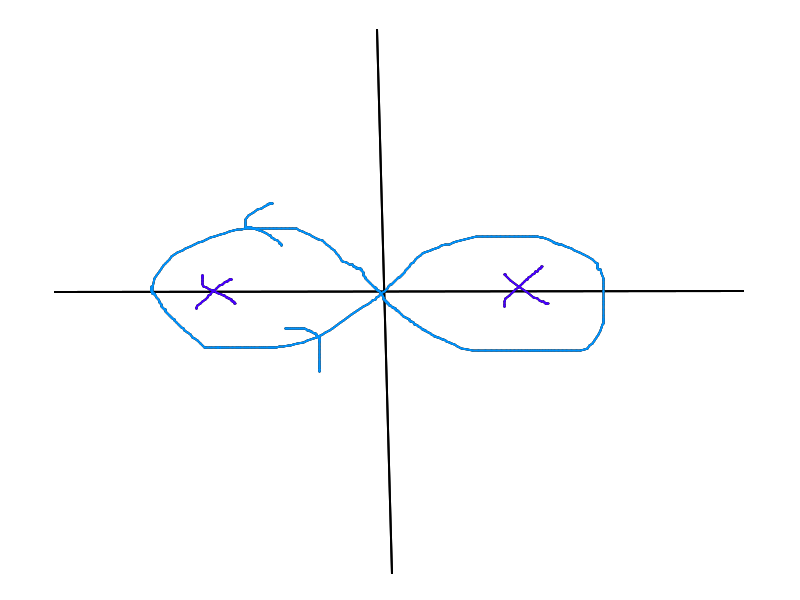
\includegraphics[width=0.7\linewidth]{leg_2}
	\caption{Contour of Legendre function of the second kind. It is ok to do this kind of contour since the multi-valuedness cancels out.}
	\label{fig:leg2}
\end{figure}

$Q_\nu(z)$ is a L.I. solution of Legendre equations such that $P_\nu, Q_\nu$ provide a fundamental set.

\subsection{Bessel Functions}
Using separation of variables (e.g. for Helmholtz equation) leads to Bessel's equation:

\begin{align}\label{eq:bes}
z^2 w'' + z w' + (z^2-\nu^2)z=0,\ \nu \in \C
\end{align}

We note that this function has regular singular point at $z=0$, however the point $z=\infty$ is not a regular singular point. Since the only singularity in the finite plane is at $z=0$, solutions are expected to be entire except for the branch point at $z=0$. Therefore, look for solutions of the form 

\begin{align*}
w=z^\rho (a_0 - a_1z + a_2z^2...)
\end{align*}

We plug this into the Bessel Equation (Equation \ref{eq:bes}). We find the first equation is:

\begin{align}\label{eq:besses}
a_0(\rho^2-\nu^2&)=0 \\ 
a_1[(\rho+1)^2-\nu^2] &= 0 \\ 
a_2[(\rho+2)^2-\nu^2] &= -a_0 \\ 
a_n[(\rho+n)^2-\nu^2] &= -a_{n-2}
\end{align}

The indicial equation is $\rho = \pm \nu $. We denote $\rho_1 = +\nu$ to be the root with the largest real part. $\rho_2 = -\nu$ is the second root. Then we choose $\rho = +\nu$ in Equation \ref{eq:besses}.  None of the $a$ coefficients vanishes and we always have a solution of the form:

\eq{1+\frac{1}{1-(\nu+1)} \left(\frac{z}{2}\right)^2 +\frac{1}{2(\nu+1)(\nu+2)}\left(\frac{z}{2}\right)^4+... }


Conventionally, we get:

\begin{align*}
a_0 = \frac{1}{2^\nu \Gamma(\nu+1)}
\end{align*}

\begin{align*}
J_\nu (z) = \left(\frac{z}{2}\right)^\nu \sum_{n=0}^{\infty} \frac{(-1)^n}{n! \Gamma(\nu+n+1)} \left(\frac{z}{2}\right)^{2n}
\end{align*}
This is called \textbf{Bessel's equation of the first kind} (of order $\nu$).
\textbf{Note:} Apart from the factor $\left(\frac{z}{2}\right)^0$, the power series has an infinite radius of convergence, so that $\left(\frac{z}{2}\right)^{-\nu}J_\nu(z)$ is entire.

For \textit{integer} $\nu=n>0$, then the Bessel function has the property:

\begin{align*}
J_n(z) = \left(\frac{z}{2}\right)^\nu \left[\frac{1}{0!n!} - \frac{1}{1!(n+1)!}\left(\frac{z}{2}\right)^{2}+...\right] 
\end{align*}

This is called the Bessel Coefficient of order n. It is an entire function.

\textbf{Note:} If the difference between indicial roots $2\nu$ is not an integer, the choice of $\rho=-\nu$ leads to a 2nd linearly independent solution $J_{-\nu}$ Even when $2\nu$ is an odd integer, $J_\nu$ and $J_{-\nu}$ are linearly independent. 

We note since $2\nu = 2n$, then, the only case left is when $\nu = n \geq 0$. Then, one solution is still $J_n$ as given above. The choice $\rho=-\nu$ leads to $J_{-n}(z) = (-1)^n J_n(z)$. This does not provide a linearly independent solution.  This also suggests considering:

\begin{align*}
\lim_{\nu\to n} = \frac{J_\nu(z) - (-1)^nJ_{-\nu}(z)}{\nu-n}
\end{align*}

Which leads to the function of the second kind:

\begin{align*}
Y_{\alpha }(x)={\frac {J_{\alpha }(x)\cos(\alpha \pi )-J_{-\alpha }(x)}{\sin(\alpha \pi )}}
\end{align*}


When $\nu \neq n$, $Y_\nu$ is linearly independent from $J_\nu$. In the limit as $\nu \to n$, 

\begin{align*}
Y_n(z) = \frac{1}{\pi}  \left[\pdv{J_\nu}{\nu} - (-1)^n \pdv{J_{-\nu}}{\nu}  \right]_{\nu=n}
\end{align*}

And this is linearly independent from $J_n$. For the case $n\geq 0$, we get:

\begin{align*}
 Y_{n}(z)=-{\frac {\left({\frac {z}{2}}\right)^{-n}}{\pi }}\sum _{k=0}^{n-1}{\frac {(n-k-1)!}{k!}}\left({\frac {z^{2}}{4}}\right)^{k}+{\frac {2}{\pi }}J_{n}(z)\ln {\frac {z}{2}}-{\frac {\left({\frac {z}{2}}\right)^{n}}{\pi }}\sum _{k=0}^{\infty }(\psi (k+1)+\psi (n+k+1)){\frac {\left(-{\frac {z^{2}}{4}}\right)^{k}}{k!(n+k)!}}
\end{align*}

Where $\phi(z)$ is the digamma function.

% final exam is friday 13th 

\Section{Caucy Data on Arbitrary Curve $\Gamma$}
Let $\Gamma$ be defined by 
\eq{\xi (x,y) = 0}

and define adjacent curves $\xi(x,y) = $constant. We also defined a family:

\eq{\eta(x,y)= \text{constant}}

This is defined in such a way that $\xi, \eta$ define a log coordinate system:

\begin{align*}
J(x,y) = \xi_x \eta_y - \xi_y \eta_x \neq 0
\end{align*}

The cauchy data on $\Gamma$ prescribe $\phi$ and normal derivative $\dv{\phi}{m}$ on $\Gamma$. Can we compute $\phi_{\eta \eta}, \phi_{\eta \xi }, \phi_{\eta \eta \xi},...$ in order to find $\phi_{\xi \xi }$ from the PDE:


\begin{align*}
A \phi_{xx} + B \phi_{xy} + C \phi_{yy} + D \phi_{x} + E \phi_{y} + F \phi + G = 0
\end{align*}

 We have to make a change of variables $(x,y) \to (\xi, \eta)$. We note that $\phi_x = \phi_\xi \xi_z + \phi_\eta \eta_x$ and that $\phi_{xx} = \phi_{\xi \xi} \xi_x^2 + 2 \phi_{} \phi_x \eta_x + \phi_{} \eta_x^2 + \phi_{\xi} \xi_{xx} + \phi_{\eta}\eta_{xx}$

The PDE now becomes:

\begin{align*}
(A \xi_x^2 + 2 B \xi_x \xi_y + C \xi_y^2) \phi_{xx} + 2 (stuff) \phi_{\xi \eta }+ (stuff)\phi_{\eta \eta} + ... + \sigma = 0
\end{align*}

Now, in order to be able to solve for $\phi_{\xi \xi }$ in terms of $\phi_{\eta}, \phi_{\xi}, \phi_{\xi \eta}, \phi_{\eta \eta} ...$ it is necessarily that the coefficient exist:

\begin{align*}
A \xi_x^2 + 2 B \xi_x \xi_y + C \xi_y^2 \neq 0
\end{align*}

On the other hand, if the left hand side = 0, then the procedure fails. We note the coefficient can be written as


\begin{align*}
A \left(\frac{\xi_x}{\xi_y}\right)^2 + 2 B \left(\frac{\xi_x}{\xi_y}\right)^2 + C = 0
\end{align*}

This is quadratic in $\frac{\xi_x}{\xi_y}$. The solution depends on the discriminant $B^2-AC$. There are three cases: 

\underline{\textbf{Case 1:} $B^2-AC>0$}

In this case, 
	\begin{align*}
	\frac{\xi_x}{\xi_y} = \frac{-B\pm \sqrt{B^2-AC}}{A}
	\end{align*}
	
	Now, on $\xi(x,y) = const$, we get 
	\begin{align*}
	\dv{y}{x} = - \frac{\xi_x}{\xi_y}
	\end{align*}
	
	From this, we conclude that the Cauchy data is insufficient on any curve for which:
	
	\begin{align}\label{eq:d1}
	\dv{y}{x} = \frac{B + \sqrt{B^2-AC}}{A}
	\end{align}
	
	\begin{align}\label{eq:d2}
	\dv{y}{x} = \frac{B - \sqrt{B^2-AC}}{A}
	\end{align}
	
	These curved can be obtained by integration and are called \textbf{characteristics.} We choose Equation \ref{eq:d1} to define $\xi(x,y) = const$ and Equation \ref{eq:d2} to define $\eta(x,y) = const$. We note that these equations are never tangent.
	
	\textbf{Note: } In this special coordinate system, the PDE becomes:
	
	\begin{align*}
	\phi_{\xi \eta} +\alpha + \phi_\xi + \beta + \phi_\eta + \gamma \phi + \delta = 0
	\end{align*}
	
	We note that if $B^2-AC>0$ in a region, the PDE is hyperbolic. In this case, there are 2 families of characteristics. 
	
	\begin{ex}[Wave Equation]
		Given:
		
		\begin{align*}
		\frac{1}{c^2}\phi_{tt}= \phi_{xx}
		\end{align*}
		
		This has the characteristic:
		
		\begin{align*}
		\xi = x + ct \\ 
		\eta = x - ct
		\end{align*}
		
		The PDE becomes:
		
		\begin{align*}
		\phi_{\xi \eta} &= 0 \\ 
		\phi(\xi, \eta)& = F(\xi) G(\eta)
		\end{align*}
	\end{ex}

\underline{\textbf{Case 2:} $B^2 - AC = 0$}

Without loss of generality, we take $A\neq 0$. (If $A=0$, take $C\neq 0$). Then, 

\begin{align*}
\frac{\xi_x}{\xi_y} = -\frac{B}{A} = - \dv{y}{x}
\end{align*}

In this case, there is only one family of characteristics, or $\xi(x,y) = \text{const}$. Then the equation is said to be \textit{parabolic}. The canonical form is:

\begin{align*}
\phi_{\eta \eta} + \alpha \phi_\xi + \beta \phi_\eta + \gamma \phi + \delta = 0
\end{align*}

\begin{ex}[Diffusion Equation]

\begin{align*}
\phi_x = a^2 \phi_{xx}
\end{align*}
\end{ex}

\underline{\textbf{Case 3:} $B^2-AC < 0$}

In the region there is no characteristic and the PDE is elliptic.

\begin{ex}[Laplace's Equation]
\begin{align*}
\phi_{xx} + \phi_{yy} = 0
\end{align*}
\end{ex}

\Section{Fourier Transform }

\Def{Fourier Transform}{Given a function $f(t)$, the Fourier transform $F(\lambda)$ on $\hat{f}(\lambda)$ is defined by:

\begin{align*}
F(\lambda) = \frac{1}{\sqrt{2\pi}} \int_{-\infty}^{\infty} e^{i \lambda \tau} f(\tau) d\tau
\end{align*}

We note that $F(\lambda)$ is an analytic function. This makes it very powerful! We can use it to convert PDE to ODE, or rather an ODE of the Fourier transform.
}

\subsection{Common Fourier Transforms}
\begin{figure}[H]
	\centering
	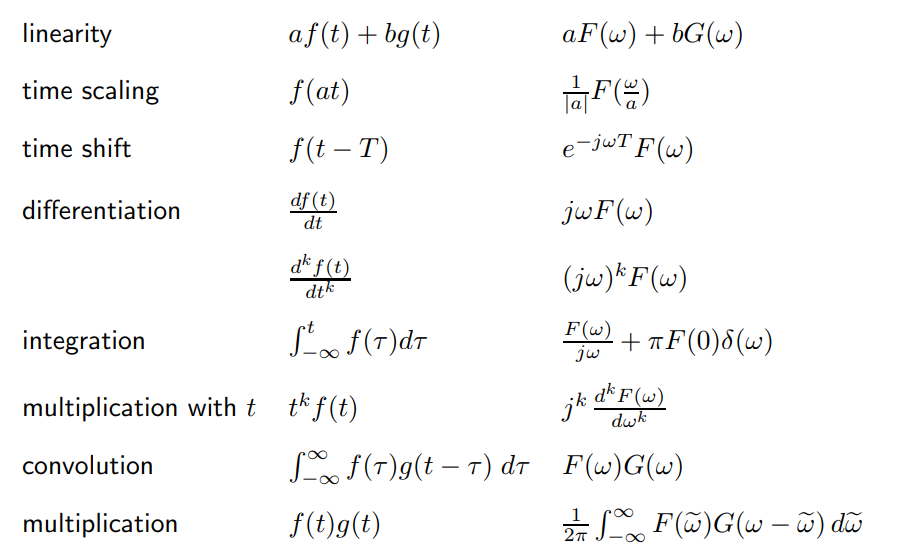
\includegraphics[width=0.7\linewidth]{common_fourier}
	\caption{Common Fourier Transforms}
	\label{fig:commonfourier}
\end{figure}


\subsection{Heuristic for Fourier Transform Inversion Formula}
Recall the Fourier series representation. A function $f(t)$, assumed to be square integrable (L2 integrable), defined on an interval $t \in [-T,T]$, has a Fourier series expansion representation given by:

\begin{align*}
f(t) &= \frac{a_0}{2} + \sum_{n=1}^{\infty} \left(a_n \cos \left(\frac{n \pi t}{T}\right) + b_n \sin \left(\frac{n \pi t}{T}\right) \right)  \\ 
a_n &= \frac{1}{T} \int_{-T}^{T} f(\tau) \cos \left(\frac{n \pi \tau}{T}\right) d\tau \\
b_n &= \frac{1}{T} \int_{-T}^{T} f(\tau) \sin \left(\frac{n \pi \tau}{T}\right) d\tau \\
\end{align*}

If we combine the results, we get that:

\begin{align*}
f(t) & = \frac{1}{2T} \int_{-T}^T f(\tau) d\tau + \sum_{n=1}^{\infty} \frac{1}{T} \int_{-T}^T f(\tau) \cos \left(\frac{n \pi }{T}\right) (\tau-t) d\tau \\ 
 &= \sum_{n=-\infty}^{\infty} \frac{1}{2T} \int_{-T}^T f(\tau) \cos \left(\frac{n \pi }{T}\right) (\tau-t) d\tau 
\end{align*}

Let $\frac{n \pi }{T} = \lambda_n$, and $\frac{\pi}{T} = \lambda_{n+1} -\lambda_n = \delta \lambda_n$. Then, we get:

\begin{align*}
f(t) &= \frac{1}{2\pi}\sum_{n=-\infty}^{\infty} \delta \lambda_n \int_{-T}^T f(\tau) \cos \lambda_n (\tau-t) d\tau 
\end{align*}

As we let $n, T \to \infty$:


\begin{align*}
f(t) &= \frac{1}{2\pi}\int_{-\infty}^{\infty}  \int_{-\infty}^\infty f(\tau) \cos \lambda (\tau-t) + d\tau d\lambda \\ 
 &= \frac{1}{2\pi}\int_{-\infty}^{\infty}  \int_{-\infty}^\infty f(\tau) \left[\cos \lambda (\tau-t) + i\sin \lambda (\tau-t) \right]d\tau d\lambda \\
 &= \frac{1}{2\pi}\int_{-\infty}^{\infty}  \int_{-\infty}^\infty f(\tau) e^{i\lambda \tau} e^{-i\lambda t}d\tau d\lambda 
\end{align*}

Therefore,
\begin{align*}
f(t) &= \frac{1}{\sqrt{2\pi}} \int_{-\infty}^\infty F(\lambda) e^{-i\lambda \tau} d\lambda 
\end{align*}

This is the \textbf{Fourier Inversion Formula}, or \textbf{Inverse Fourier Transform\\
}

\begin{theorem}
Assume that $f(t)$ is a real, piecewise-smooth function with $\int_{-\infty}^{\infty} |f(t)| dt < \infty $. 

Then, 

\begin{align*}
\lim_{L \to \infty } \frac{1}{2 \pi } \int_{-L}^{L} \int_{-\infty}^{\infty} f(\tau) \cos \lambda (\tau - t) dt d\lambda = \frac{1}{2} \left[f(t_+) + f(t_-)\right]
\end{align*}

Where:

\begin{align*}
f(t_+) = \lim_{\epsilon \to 0} f(t + \epsilon) \\ 
f(t_-) = \lim_{\epsilon \to 0} f(t - \epsilon)
\end{align*}



\Def{Piecewise smooth:} {$f$ and $f'$ are continuous in any finite interval are continuous in any finite interval, except at any finite number of discontinuities.}

\end{theorem}

\begin{lemma}
Under certain hypothesis on real, piecewise-smooth $f$, then:

\begin{align*}
\lim_{L \to  \infty} \int_{-T}^{T} f(t + \tau) \frac{\sin L\tau}{\tau} 
= \frac{\pi}{2} \left[f(t_+) + f(t_-)\right]
\end{align*}

This is related to the fact for delta functions:


\begin{align*}
\int_{-\infty}^{\infty} f(t - \tau) \delta(\tau) d\tau = f(t)
\end{align*}

The reason we can think of this is thinking of a Gaussian that becomes infinitely thin and tall as the limit of the Gaussian. The $\frac{\sin L\tau}{\tau} $ is a sort of approximation of a delta function.
\end{lemma}

% 12-2
We note that since $\sin \lambda (\tau-t)$ is odd in $\lambda$, the Fourier inversion theorem can also be written as:

\begin{align*}
\frac{1}{2\pi} \int_{-\infty}^\infty \int_{-\infty}^\infty f(\tau) e^{i \lambda (\tau - t)}  d\tau d\lambda 
=\frac{1}{2} \left(f(t_+) + f(t_-)\right) 
\end{align*}

We can rewrite this using the definition of the Fourier transform:

\begin{align*}
F(\lambda) = \frac{1}{\sqrt{2\pi}} \int_{-\infty}^\infty e^{i \lambda \tau} f(\tau) d\tau
\end{align*}
This provides the inversion formula:

\begin{align*}
\frac{1}{2} \left(f(t_+) + f(t_-)\right) = \frac{1}{\sqrt{2\pi}} \int_{-\infty}^\infty e^{i \lambda \tau} f(\tau) d\tau
\end{align*}

Note, there are other possible definitions, and that $f(t)$ need not be real valued.

\subsection{Properties of the Fourier Transform}
For a function $f(t)$ with Fourier Transform $F(\lambda)$
\begin{itemize}
	\item $I.F.T.[f(t)] = F(-\lambda)$
	\item For constants $a,b$: $F.T.[af(t)+bg(t)] = a F.T.[f(t)] + b F.T.[g(t)] $
	\item $F.T.[f(t)g(t)] = F.T.[f(t)] * F.T.[g(t)]$  where $*$ is the convolution operator.
	\item $F.T.[f(t) * g(t)] = F.T.[f(t)] F.T.[g(t)]$
	\item $F.T.[\dv{^n}{t^n} f(t)] = (-i\lambda)^n F(\lambda)$
	\item $F.T.[\delta(t)] = \frac{1}{\sqrt{2\pi}}$
	\item $F.T.[1] = \frac{1}{\sqrt{2\pi}}\delta(-t) = \frac{1}{\sqrt{2\pi}}\delta(t)$
	\item $F.T.[f(t-t_0)] = \frac{1}{\sqrt{2\pi}}  \int_{-\infty}^\infty e^{i \lambda t} f(t-t_0) dt = \frac{1}{\sqrt{2\pi}}  \int_{-\infty}^\infty e^{i \lambda (t'+t_0)} f(t') dt' = e^{i \lambda t_0} F(\lambda)$
\end{itemize}

\subsection{Extensions of Fourier}
The theorem does not say that the inversion result is not valid under more general hypotheses. As an example of a non-working inversion:

\begin{align*}
g(t) = \begin{cases}
t^{-1/2} &t > 0 \\ 
0 & t < 0
\end{cases}
\end{align*}
\begin{align*}
\int_{-\infty}^{\infty} \left|g(t)\right| dt = \int_{0}^{\infty} \frac{1}{\sqrt{t}} dt = 2 \sqrt{t} |_0^\infty \to \infty 
\end{align*}
Hence, the theorem does not guarantee inversion.

However, contour integration can be used to show:

\begin{align*}
G(\lambda) &= \frac{1}{\sqrt{2 \pi }} \int_{-\infty}^{\infty} e^{i \lambda \tau } \tau^{-1/2} d\tau \\
 &=  \frac{1}{\sqrt{\lambda}} \left(1 + i \frac{\lambda}{|\lambda|}\right),\ \lambda \in \R^+, \lambda \neq 0
\end{align*}

Can we invert $G(\lambda)$ to get back $g(t)$. This does in fact work:

\begin{align*}
\frac{1}{\sqrt{2\pi}}\int_{-\infty}^{\infty} G(\lambda) e^{i\lambda t} d\lambda = g(t)
\end{align*}

Thus, the inversion results works even though the hypothesis of the Fourier Inversion Theorem are not satisfied. What is the moral of this story? We must try to see if it works.

\begin{ex}
\begin{align*}
f(t) = \begin{cases}
t^{1/2} &t > 0 \\ 
0 & t < 0
\end{cases}
\end{align*}

Then, 

\begin{align*}
F(\lambda) = \frac{1}{\sqrt{2\pi}}\int_{-\infty}^{\infty} t^{1/2} e^{i\lambda t} dt
\end{align*}

But this integral does not make sense. It does not converge for $\lambda \in \R$. However, the integral converges when $\Im{\lambda} > 0$. For such a $\lambda$, in fact, it can be shown that $F(\lambda) = \frac{1}{2\sqrt{2}} e^{-i\frac{3\pi}{4}} \lambda^{-\frac{3}{2}}$ for $0 < \arg \lambda < \pi$. By analytic continuation, this definition can be extended to the complex plane, except for $\lambda = 0$. 

Next, we write $\lambda = \lambda_1 + i \lambda_2$, where $\lambda_1, \lambda_2 \in \R$. If we hold $\lambda_2 > 0$ fixed, we can then define $G(\lambda_1) = F(\lambda_1 + i \lambda_2)$. This is the Fourier transform of $g(t) = e^{-\lambda_2 t} f(t)$ for $\lambda_1 \in \R$. Then, by the Fourier Inversion Theorem:

\begin{align*}
g(t) = \frac{1}{\sqrt{2\pi}}\int_{-\infty}^{\infty}  e^{i\lambda_1 t} G(\lambda_1) d\lambda_1
\end{align*}

Additionally, 
\begin{align*}
f(t) &= e^{\lambda_2 t} g(t) \\ 
&= \frac{1}{\sqrt{2\pi}}\int_{-\infty+i\lambda_2}^{\infty+i\lambda_2}  e^{\lambda t} F(\lambda) d\lambda
&= \frac{1}{\sqrt{2\pi}}\int_\Gamma  e^{\lambda t} F(\lambda) d\lambda
\end{align*}

We have now turned this into a contour integral along the real line with contour $\Gamma$. It can be checked that the inversion formula does in fact work.

\end{ex}


\subsection{Sine and Consine Transform}

Often, $f(t)$ is defined for $t>0$. Then, it is useful to extend $f$ such that $f(-t) = f(t)$ (i.e., $f$ is even). Then the following is also even:

\begin{align*}
F(\lambda) = \frac{1}{\sqrt{2\pi}}\int_{-\infty}^{\infty}  e^{i\lambda \tau} f(\tau) d\tau\\
F(-\lambda) = F(\lambda)
\end{align*}

And so we can write the cosine and sine transformation:
\Def{Cosine Transformation}{
	
We can consider the cosine Fourier transform of $f$:
\begin{align*}
F_c(\lambda) = \sqrt{\frac{2}{\pi}} \int_{0}^{\infty} (\cos \lambda \tau ) f(\tau) d\tau
f(t) = \sqrt{\frac{2}{\pi}} \int_{0}^{\infty} (\cos \lambda \tau ) F_c(\lambda) d\lambda
\end{align*}
}

\Def{Sine Transformation}{
	
	We can consider the cosine Fourier transform of $f$:
	\begin{align*}
	F_s(\lambda) = \sqrt{\frac{2}{\pi}} \int_{0}^{\infty} (\sin \lambda \tau ) f(\tau) d\tau
	f(t) = \sqrt{\frac{2}{\pi}} \int_{0}^{\infty} (\sin \lambda \tau ) F_s(\lambda) d\lambda
	\end{align*}
}

\subsection{Fourier transform of derivatives}

Consider functions $f$ that vanish as $|t| \to \infty$. Then, 

\begin{align*}
F_1(\lambda) &= F.T. \{f'\}\\
& = \frac{1}{\sqrt{2 \pi}} \int_{-\infty}^{\infty}  e^{i\lambda t} f'(t) dt
\end{align*}

By integration by parts:

\begin{align*}
F_1(\lambda) & = \frac{1}{\sqrt{2 \pi}} \left[e^{i\lambda t} f(t) \right]_{-\infty }^\infty - i \lambda \int_{-\infty}^{\infty}  e^{i\lambda t} f(t) dt
&= (-i\lambda) F(\lambda)
\end{align*}

Similarly, the Fourier transform of higher derivatives $f^{(n)}(t)$ , this is given by:

\begin{align}
F_n(\lambda) = F.T. \{f^{(n)}(t)\} = (-i\lambda)^n F(\lambda)
\end{align}

Note, this result is most useful for ODEs and PDEs.

\begin{ex}[1-D Conductivity]
\begin{align*}
\frac{1}{\alpha} \pdv{\phi}{t} = \pdv{ ^2 \phi}{x^2}
\end{align*}

We need to find $\phi(x,t)$ satisfying initial conditions $\phi(x,0) = g(x)$ and boundary condition $\phi(x,t) \to 0$ as $|x| \to \infty$. 

Thus, we define a Fourier transform of $\phi$ with respect ot $x$:

\begin{align*}
\Phi(\lambda, t) = \frac{1}{\sqrt{2 \pi}} \int_{-\infty}^{\infty}  e^{i\lambda x} \phi(x,t) dx
\end{align*}

Then, let us multiply the PDE by $\frac{1}{\sqrt{2 \pi}}  e^{i\lambda x}$. Then, we can integrate. We get:

\begin{align*}
\pdv{\Phi(\lambda, t)}{t} = \alpha (-i\lambda)^2\Phi(\lambda, t)
\end{align*}

We note, that we interchanged diff with respect to $t$ and integrated in r.t. x. This is an assumption that can be verified after the fact.

Note, we transformed the PDE in two variables into an ODE in one variable. The Form of the ODE is:

\begin{align*}
\Phi(\lambda, t) = A(\lambda) e^{-\alpha \lambda^2 t}
\end{align*}
where $A(\lambda)$ is an unknown function to be defined from the initial conditions. Thus, for $t=0$, we have:

\begin{align*}
A(\lambda) = \Phi(\lambda, 0) = \frac{1}{\sqrt{2 \pi}} \int_{-\infty}^{\infty}  e^{i\lambda x} \phi(x,t) dx
\end{align*}

We let $g(x) = \phi(x,t)$. Then, let $g(x) = B e^{-\beta x^2}$. We get:

\begin{align*}
A(\lambda) = \Phi(\lambda, 0) = \frac{B}{\sqrt{2 \pi}} \int_{-\infty}^{\infty}  e^{i\lambda x - \beta x^2} dx
&= \frac{B}{\sqrt{2 \pi}}  e^{-\frac{\lambda^2}{4\beta}}
\end{align*}

We can complete the square to get:

\begin{align*}
e^{-\frac{\lambda^2}{4\beta}} \int_{-\infty}^\infty e^{-\beta (x + \lambda / (2\beta))^2} dx = e^{-\frac{\lambda^2}{4\beta}} \sqrt{\frac{\pi}{\beta}}
\end{align*}

We do the integration and get:

\begin{align*}
\phi(x,t) = \frac{B}{\sqrt{\beta \pi}} \int_{-\infty}^\infty e^{- i \lambda x-\lambda^2 (1/(4\beta) + x t)} dt 
\end{align*}

And by completing the square: 
\begin{align*}
\phi(x,t) = \frac{B}{\sqrt{1 + 4 \alpha \beta t}} e^{-\frac{\beta x^2}{1 + 4 \alpha \beta t}}
\end{align*}

We can check the initial and boundary conditions.

\end{ex}

% 12-4

\section{Convolution Integrals}

\Def{Convolution}{
The convolution of $f$ and $g$ is defined as :

\begin{align*}
f \conv g = \frac{1}{\sqrt{2 \pi}} \int_{-\infty}^{\infty} f(\xi) g(x - \xi) d\xi
\end{align*}

}

We not that there is no general form for the Fourer transform of the product of $f$ and $g$:

\begin{align*}
\F (f \cdot g) \neq \F (f) \F (g)
\end{align*}

However:
\begin{align}
\F (f * g) &= \F(f) \F (g) \\ 
& = F(\lambda ) G(\lambda)
\end{align}

\textbf{Proof:}

Consider the inverse Fourier transform of $F(\lambda ) G(\lambda)$:

\begin{align*}
\frac{1}{\sqrt{2 \pi}} \int_{-\infty}^{\infty} e^{- i \lambda x}F(\lambda ) G(\lambda) d\lambda  &= \frac{1}{2 \pi} \int_{-\infty}^{\infty} e^{- i \lambda x}F(\lambda ) \int_{-\infty}^{\infty} e^{- i \lambda \xi}G(\lambda ) d\xi d\lambda  \\ 
& = \frac{1}{2 \pi} \int_{-\infty}^{\infty} d \xi g(\xi) \int_{-\infty}^{\infty} d\lambda e^{- i \lambda (x-\xi)}F(\lambda ) \\ 
& = \frac{1}{\sqrt{2 \pi}} \int_{-\infty}^{\infty} d \xi g(\xi) f(x-\xi) \\
& = \frac{1}{\sqrt{2 \pi}} f * g 
\end{align*}

Therefore:

\begin{align*}
\F (f * g) = F.T. \left[\frac{1}{\sqrt{2 \pi}} \int_{-\infty}^{\infty} g(\xi) f(x-\xi) d\xi\right] = F(\lambda ) G(\lambda)
\end{align*}

As a note, if we set $x=0$, then we get that:

\begin{align*}
 \int_{-\infty}^{\infty} F(\lambda) G(\lambda) d\lambda =  \int_{-\infty}^{\infty} f(x) g(-x)dx \\
  \int_{-\infty}^{\infty} F(\lambda) G(-\lambda) d\lambda =  \int_{-\infty}^{\infty} f(x) g(x)dx 
\end{align*}

Now, if we replace $g(x)$ with $g^* (x)$, then we get:
\begin{align*}
 \int_{-\infty}^{\infty} F(\lambda) G^*(\lambda) d\lambda =  \int_{-\infty}^{\infty} f(x) g^*(x)dx 
\end{align*}

If we let $f = g$, then we get \textbf{Parseval's theorem}:

\begin{align*}
 \int_{-\infty}^{\infty} |F(\lambda)|^2 d\lambda =  \int_{-\infty}^{\infty} |f(x)|^2dx 
\end{align*}

This is analogous to \textbf{Parseval's identity for Fourier series:}

\begin{align*}
\frac{1}{T} \int_{-T}^{T} f^2(t) dt = \frac{1}{2} a_0^2  + \sum_{n=1}^\infty (a_n^2 + b_n^2)
\end{align*}


We note that $x^n f(x)$ is a special equation:

\begin{align*}
\frac{1}{\sqrt{2 \pi}} \int_{-\infty}^{\infty} e^{- i \lambda x} x^n f(x) dx &= 
\left(\frac{1}{i}\right)^n \dv{^n}{\lambda^n} \left[\frac{1}{2\pi} \int_{-\infty}^{\infty} e^{- i \lambda x} f(x) dx\right] \\ 
& = (-i)^n \dv{^n}{\lambda^n} F(\lambda)
\end{align*}

We also note these transforms are great for linear equations, but cannot really be used on nonlinear equations. It is not a general method for PDEs.

\begin{ex}[Bessel's Equation]
\begin{align*}
xy'' + y' + xy = 0
\end{align*}
The Fourier transform is:
\begin{align*}
-i \dv{\lambda} \left(- \lambda^2 Y\right) - i \lambda Y - i \dv{Y} = 0
\end{align*}

We have gone from a 2nd order ODE to a first order ODE. This is simpler, since we can always integrate first order equations. This implies:

\begin{align*}
Y(\lambda) = B(1-\lambda^2)^{-1/2}
\end{align*}

where $B$ is a constant. Inverting this leads to the integral representation of Bessel's Function $J_0(x)$:

\begin{align*}
J_0(x) = \frac{B}{\sqrt{2\pi}} \int_{-\infty}^{\infty} e^{- i \lambda x}(1-\lambda^2)^{-1/2} d\lambda 
\end{align*}
\end{ex}


\Def{Delta Function}{
Consider a function 
\begin{align*}
f_\epsilon(x) = \frac{1}{\sqrt{\pi \epsilon }} e^{-\frac{x^2}{\epsilon}}
\end{align*}
where

\begin{align*}
 \int_{-\infty}^{\infty} f_\epsilon(x)  dx = 1
\end{align*}

If we take the limit as $\epsilon \to 0$, we will get the Dirac function:

\begin{align*}
f_0(x) = \begin{cases}
0 & x \neq 0\\
\infty & x = 0 
\end{cases}
\end{align*}

However, we still satisfy:
\begin{align*}
\int_{-\infty}^{\infty} f_0(x)  dx = 1
\end{align*}



\begin{figure}[H]
	\centering
	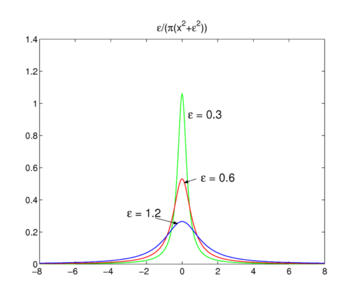
\includegraphics[width=0.7\linewidth]{eps_dirac}
	\caption{Example of how a Gaussian changes as we shrink $\epsilon$. }
	\label{fig:epsdirac}
\end{figure}

This is a physical unit impulse. This is not a real function, but it is very useful. We call $f_0(x)$ a generalization function on a distribution:

\begin{align*}
\delta(x) = \lim_{\epsilon \to 0} f_\epsilon(x)
\end{align*}
with the property:
\begin{align*}
\int_{-\infty}^{\infty} g(x) \delta(x-a)  dx = g(a)
\end{align*}

}

There is a formal procedure here, but we can make it rigorous by thinking of a $\delta$ function as a functional, or linear operator, that localizes the value of the function at point $x=a$.

\textbf{Properties of $\delta$ function:}
\begin{itemize}
	\item $\delta(-t) = \delta(t)$ 
	\item $\delta(at) = \frac{1}{|a|}\delta(t)$
	\item $t\delta(t) = 0$
	\item $\delta(t^2 - a^2) = \frac{1}{2|a|}\left[\delta(t+a) + \delta(t-a)\right]$
	\item $\delta(t) = -t \delta ' (t) \ (I.B.P.)$
\end{itemize}

The Fourier transform of $\delta(t)$ is:

\begin{align*}
F(\delta) = \frac{1}{\sqrt{2\pi}} \int_{-\infty}^{\infty} e^{- i \lambda t} \delta(t) dt  = \frac{1}{\sqrt{2\pi}} 
\end{align*}

If we let $g(t) = \delta(t-a)$, the Fourier transform of $g(t)$ is 

\begin{align*}
G(\lambda) = \frac{1}{\sqrt{2\pi}} \int_{-\infty}^{\infty} e^{- i \lambda t} \delta(t-a) dt  = \frac{1}{\sqrt{2\pi}} e^{i \lambda a}
\end{align*}

The inversion is:

\begin{align*}
g(t) &=  \frac{1}{\sqrt{2\pi}} \int_{-\infty}^{\infty}\frac{1}{\sqrt{2\pi}} e^{- i \lambda t}  e^{i \lambda a} d\lambda \\ 
&= \frac{1}{2\pi(a-t)} e^{- i \lambda (a-t)} 
\end{align*}

In short:
\begin{align*}
\frac{1}{2\pi} \int_{-\infty}^{\infty} e^{- i \lambda( a-t)} d\lambda = \delta(t-a) 
\end{align*}

\begin{ex}
For $x \in (-\infty, \infty), t > 0$:
\begin{align*}
\pdv{\phi}{t} = \alpha \pdv{^2\phi}{x^2} 
\end{align*}

We remember that:

\begin{align*}
f(x) = \int_{-\infty}^{\infty}f(\xi)\delta(\xi-x) d\xi
\end{align*}

This "equals" $\delta(t-a)$. We note that $\phi(x,0) = f(x)$ and $\phi(x,t) \to 0$ as $|x| \to \infty$. By linear superposition, the solution to the above problem can be obtained from the solution $G(x,t;\xi)$ of the following problem:

\begin{align*}
\pdv{G}{t} &= \alpha \pdv{^2G}{x^2} \\
G(x,0;\xi) &= \delta(x-\xi) \\ 
G(x,t;\xi)  \to 0 &\text{ as } |x| \to \infty 
\end{align*}

This is the same problem with a slight variation. The solution is obtained by the Fourier Transform of the PDE w.r.t. x:

\begin{align*}
\hat{G}(\lambda, t;\xi) = A(\lambda)e^{-\alpha \lambda^2 t}
\end{align*}

where 

\begin{align*}
A(\lambda) & =  \frac{1}{\sqrt{2\pi}} \int_{-\infty}^{\infty} e^{- i \lambda x} \delta(x-\xi) dx \\
& =  \frac{1}{\sqrt{2\pi}} e^{- i \lambda \xi}
\end{align*}

such that:

\begin{align*}
\hat{G}(\lambda, t;\xi)  = \frac{1}{\sqrt{2\pi}} e^{- i \lambda \xi - \alpha \lambda^2 t}
\end{align*}

Inverting this, we get Green's function:

\begin{align*}
G(x,t;\xi) &=  \frac{1}{\sqrt{2\pi}} \int_{-\infty}^{\infty} e^{- i \lambda x}\hat{G} d\lambda \\& = \frac{1}{\sqrt{2\pi \alpha t}} e^{-\frac{|x-\xi|^2}{4 \alpha t}} \\ 
& = G(x-\xi, t; 0)
\end{align*}
\end{ex}
% 12-9 - need to ask walker to fill in

\subsection{Fourier Transform in 3D}
Given the problem of Laplace's equation in 3D:
\begin{align*}
\pdv{^2\phi}{x^2} + \pdv{^2\phi}{y^2} + \pdv{^2\phi}{z^2} = g(x)
\end{align*}

With boundary conditions $\phi(\mathbf{x}) \to 0$ as $|\mathbf{x}| \to \infty$. 

\Def{Fourier Transform in 3D}{
For a function $f$, the Fourier transform is:

\begin{align*}
F(\mathbf{\lambda}) = \frac{1}{(2 \pi)^{3/2}} \iiint_{-\infty}^\infty e^{i \mathbf{\lambda x}} f(\mathbf{x}) dv_\mathbf{x}
\end{align*}
}

Now let's think about the second derivative Fourier transform in 3D:

\begin{align*}
G(\lambda_1, \lambda_2, \lambda_3) &= \frac{1}{(2 \pi)^{3/2}} \iiint_{-\infty}^\infty e^{i (\lambda_1 x \lambda_2 y \lambda_3 z)} \pdv{^2 f(x,y,z)}{x} dxdydz \\ 
&= -\lambda_x^2 F(\mathbf{\lambda}) -\lambda_y^2 F(\mathbf{\lambda}) -\lambda_z^2 F(\mathbf{\lambda}) \\
&= \frac{1}{(2 \pi)^{3/2}} \iiint_{-\infty}^\infty e^{i \mathbf{\lambda x}} \delta(\mathbf{x} - \mathbf{\xi}) dv\mathbf{x} \\ 
& = \frac{1}{(2 \pi)^{3/2}} e^{i \mathbf{\lambda \xi}}
\end{align*}

Now this becomes an algebraic equation, where $G$ is the Green's function:

\begin{align*}
-|\mathbf{\lambda}|^2 G(\mathbf{\mathbf{\lambda}}) = \frac{1}{(2 \pi)^{3/2}}  e^{i \mathbf{\lambda \xi}} \\
G(\mathbf{\lambda}) = \frac{1}{-(2 \pi)^{3/2}|\mathbf{\lambda}|^2}  e^{i \mathbf{\lambda \xi}} 
\end{align*}

To finish up, we do the inverse Fourier Transform:

\begin{align*}
g(\mathbf{x};\xi) = \frac{-1}{(2 \pi)^{3/2}} \iiint_{-\infty}^\infty e^{-i  \mathbf{\lambda x}} \frac{e^{-i  \mathbf{\lambda \xi}}}{|\mathbf{\lambda}|} d\frac{1}{\mathbf{\lambda}} \\ 
= \frac{-1}{(2 \pi)^{3/2}} \iiint_{-\infty}^\infty \frac{e^{-i  \mathbf{\lambda} (\mathbf{x} - \mathbf{\xi})}}{|\mathbf{\lambda}|} d\frac{1}{\mathbf{\lambda}} \\ 
\end{align*}

This has a problem where there could be a singularity at $\lambda = 0$. We can rewrite this volumetric integral making use of spherical coordinates. We do a change of variables $d \frac{1}{\lambda} = \rho^2 \sin \theta d\rho d\theta d\phi $.

We also have the vector $|\mathbf{x - \xi }| = r$. So then, we get the result:

\begin{align*}
g(\mathbf{x};\xi) = \frac{-1}{(2 \pi)^{3}} \int_{0}^{2\pi} d\phi \int_0^\infty d\rho \int_0^\pi d\theta \frac{e^{-i \rho r \cos \theta }\rho^2 \sin \theta }{\rho^2} \\
= \frac{-1}{(2 \pi)^{3}} \int_{0}^{2\pi} d\phi \int_0^\infty d\rho \int_0^\pi d\theta e^{-i \rho r \cos \theta } \sin \theta 
\end{align*}

We note the final answer does not depend on $\phi$, so we get a factor of $2\pi$.

\begin{align*}
g(\mathbf{x};\xi) = \frac{-1}{(2 \pi)^{2}}  \int_0^\infty d\rho \int_0^\pi d\theta e^{-i \rho r \cos \theta } \sin \theta 
\end{align*}

With another change of variables $u = -cos\theta$, $du = -sin\theta d\theta$:

\begin{align*}
g(\mathbf{x};\xi)&= \frac{-1}{(2 \pi)^{2}}  \int_0^\infty d\rho \int_{-1}^1  e^{i \rho r u} du \\ 
&= \frac{-1}{(2 \pi)^{2}}  \int_0^\infty d\rho \left[\frac{1}{i\rho r}\right] \left[e^{i \rho r} - e^{-i \rho r}\right]\\
&= \frac{-1}{2 (\pi)^{2} r}  \int_0^\infty d\rho \frac{1}{\rho}\sin (\rho r)\\
&= \frac{-1}{2 (\pi)^{2} r}  \int_0^\infty d(r\rho) \frac{1}{r\rho}\sin (\rho r) \\
&= \frac{-1}{2 (\pi)^{2} r}  \int_0^\infty dx \frac{1}{x}\sin x \\
& = - \frac{1}{4 \pi r}
\end{align*}

Back to the Green's function:

\begin{align*}
g(\mathbf{x};\mathbf{\xi}) = - \frac{1}{4 \pi |\mathbf{x}-\mathbf{\xi}|} \\
\phi(\mathbf{x}) = -\iiint_{-\infty}^\infty f(\mathbf{\xi}) \frac{1}{4 \pi |\mathbf{x}-\mathbf{\xi}|} dv_\mathbf{x}
\end{align*}
This is the idea of a kernel.

\subsection{Wave Equation}

The wave equation is a hyperbolic equation which can be solved with a change of variables.

\begin{align*}
\pdv{^2u}{t^2} = c^2 \pdv{^2 u}{t^2}
\end{align*}

The physical interpretation is imagine an infinite string. It has a property $c = \sqrt{T/\rho}$, where $T$ is the tension in the string and $\rho$ is mass per unit length.

We have some boundary conditions:

\begin{align*}
u(x,0) = h(x) \\ 
\pdv{u}{t}(x,0) = p(x)
\end{align*}
We also have the condition that $u \to 0$ as $|x| \to \infty$. 

A general solution for constant $c$ can easily be found by a change of variables. 

\begin{align*}
\xi = x + ct\\
\eta = x - ct 
\phi(\xi, \eta) = u(\frac{\xi + \eta}{2}, \frac{\xi - \eta}{2c})
\end{align*}

The PDE becomes:
\begin{align*}
\pdv{^\phi}{d\xi d\eta} = 0
\end{align*}

The solution to this equation is simply with $\alpha, \beta$ arbitrary functions in one variable:

\begin{align*}
\phi(\xi, \eta) = \alpha (\xi) + \beta(\eta)
\end{align*}

In terms of $x,t$, we have:
\begin{align*}
u(x,t) = \alpha(x+ct) + \beta(x-ct)
\end{align*}

In making use of the initial conditions, we get the result:

\begin{align*}
u(x,t) = \frac{1}{2}(h(x+ct) + +h(x-ct)) + \frac{1}{2c} \int_{x-ct}^{x+ct} P(\tau) d\tau
\end{align*}

Now we can consider the forced version of the wave equation:

\begin{align*}
\pdv{^2u}{t^2} = c^2 \pdv{^2 u}{t^2} + F
\end{align*}

Now we must use contour integration in order to solve this. There are two singularities along the real line, so we must do an indented path idea. But should we indent above or below? Alternatively, we can also introduce some friction:

\begin{align*}
\alpha \pdv{u}{t} + \pdv{^2u}{t^2} = c^2 \pdv{^2 u}{t^2} + F
\end{align*}

This moves the two singularities. One moves above, one moves below the real axis, solving the contour integration issue. As dissipation moves to zero, we clearly see which side we should indent on to be consistent with physics. 


% ======================================================================
\end{document}